\chapter{Nervous and immune systems as control systems}
\label{vol06:ch07}

\epigraph{The behaviour of nerve fibres can be described in terms of
the changes in membrane conductance for sodium and potassium ions,
and the resulting movement of these ions.}{Alan L.\ Hodgkin and
Andrew F.\ Huxley, \emph{Journal of Physiology} 117:500 (1952),
introductory section \cite[p.~500]{paper:v6c07-hodgkin-huxley-1952}.}

\chapmeta{Half-life: foundational. Archetypes: control, interface. Exercise target: 30. Project track: simulation (leaky integrate-and-fire neuron, reproducing simple firing patterns and refractory behaviour). Hazard class: none (in-silico work). Reader path default: standard, with sections explicitly tagged. Named cases: none required; autoimmunity, infection, and immunodeficiency are described as mechanism classes, with the COVID-19 mRNA vaccine roll-out (2020--2023), the SCID-X1 gene-therapy leukaemia incidents (2002--2003), and the thalidomide birth-defect epidemic (1957--1961) cited at paper level for engineering context.}

\noindent
The nervous and immune systems are the body's two distributed
information-processing networks. The nervous system performs fast,
local, point-to-point signalling at millisecond timescales; the immune
system performs slow, distributed, pattern-recognition-based defence
at timescales from hours to weeks. Both systems read naturally as
control systems: each has sensors, effectors, feedback loops, memory,
and characteristic failure modes. The chapter develops the neuron as a
device, the action potential as a propagating signal, the synapse as a
signal-modulation point, the nervous system as a distributed control
architecture, the immune system as a pattern-recognition-and-response
system, and the failure modes (autoimmunity, infection, and
immunodeficiency) that arise when either control system breaks.

\section{Neurons as devices}\pathtag{core}

A \engterm{neuron} is a cell specialised for the rapid, long-distance
propagation of electrical signals. Each neuron has a cell body
(\engterm{soma}), a long output process (the \engterm{axon}), and a
branching input structure (the \engterm{dendritic tree}). The soma
houses the nucleus and most of the cell's biosynthetic machinery;
the axon carries action potentials away from the soma; the dendrites
receive signals from other neurons through synaptic contacts
(Figure~\ref{fig:vol06:ch07:neuron}).

\begin{figure}[htbp]
\centering
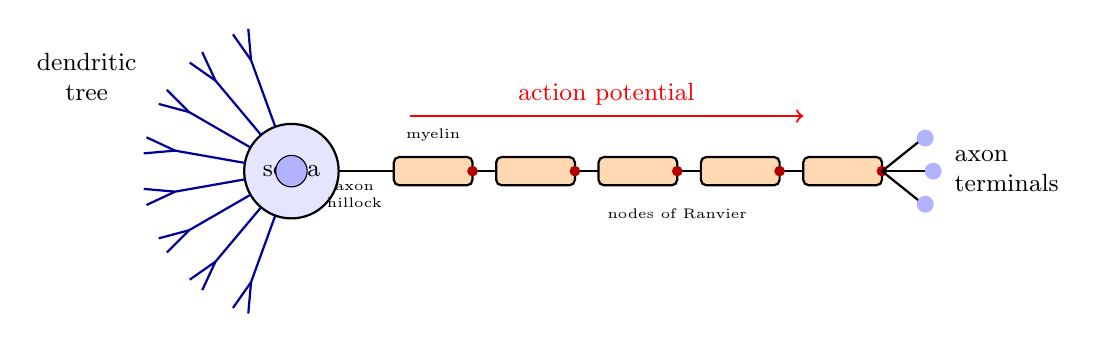
\begin{tikzpicture}[scale=1.0, every node/.style={font=\small}]
  % Soma
  \draw[thick, fill=blue!10] (0,0) circle (0.6);
  \node at (0,0) {soma};
  \draw[fill=blue!30] (0,0) circle (0.2);
  % Dendrites
  \foreach \a in {110, 130, 150, 170, 190, 210, 230, 250} {
    \draw[thick, color=blue!60!black] (\a:0.6) -- ++(\a:0.9);
    \draw[thick, color=blue!60!black] (\a:1.5) -- ++(\a+15:0.4);
    \draw[thick, color=blue!60!black] (\a:1.5) -- ++(\a-15:0.4);
  }
  \node[align=center] at (-2.6,1.2) {dendritic\\tree};
  % Axon hillock
  \draw[thick] (0.6,0) -- (1.0,0);
  \node[below, align=center, font=\tiny] at (0.8,-0.05) {axon\\hillock};
  % Axon with myelin segments
  \draw[thick] (1.0,0) -- (7.5,0);
  \foreach \x in {1.3, 2.6, 3.9, 5.2, 6.5} {
    \draw[thick, fill=orange!30, rounded corners=2pt] (\x,-0.18) rectangle (\x+1.0,0.18);
  }
  \node[above, font=\tiny] at (1.8,0.25) {myelin};
  % Nodes of Ranvier
  \foreach \x in {2.3, 3.6, 4.9, 6.2, 7.5} {
    \filldraw[red!70!black] (\x,0) circle (0.06);
  }
  \node[below, align=center, font=\tiny] at (4.9,-0.35) {nodes of Ranvier};
  % Axon terminals
  \draw[thick] (7.5,0) -- (8.0,0.4);
  \draw[thick] (7.5,0) -- (8.0,-0.4);
  \draw[thick] (7.5,0) -- (8.1,0);
  \filldraw[blue!30] (8.05,0.42) circle (0.1);
  \filldraw[blue!30] (8.05,-0.42) circle (0.1);
  \filldraw[blue!30] (8.15,0) circle (0.1);
  \node[right, align=left] at (8.3,0) {axon\\terminals};
  % Direction arrow
  \draw[->, thick, color=red] (1.5,0.7) -- (6.5,0.7) node[midway, above] {action potential};
\end{tikzpicture}
\caption[Neuron schematic]{Schematic of a vertebrate motor neuron. Dendrites
(left) integrate synaptic inputs; the soma houses the nucleus; the
axon hillock initiates the action potential; the myelinated axon
propagates the spike by saltatory conduction across nodes of Ranvier;
axon terminals release neurotransmitter onto downstream neurons or
muscle.}
\label{fig:vol06:ch07:neuron}
\end{figure}


\engterm{The membrane as a circuit.} The neuron's plasma membrane is
described by an equivalent electrical circuit. The lipid bilayer acts
as a capacitor with specific capacitance $C_m \approx 1\,\si{\micro\farad}/
\text{cm}^2$ (set by the bilayer thickness of $\sim 5\,\text{nm}$ and
the dielectric constant of the hydrocarbon interior). Ion channels in
the membrane provide conducting pathways for specific ions; each
channel type contributes a conductance whose value depends on the
channel's gating state. The result is a parallel RC network, with the
capacitance set by the bilayer geometry and the conductances set by
the channel population.

\engterm{Resting potential.} A typical neuron at rest has a membrane
potential of $-65$ to $-75\,\text{mV}$, with the inside negative
relative to the outside. The potential arises from the unequal
distribution of ions across the membrane (high potassium inside,
high sodium and chloride outside; see Chapter~\ref{vol06:ch01}) and
the selective permeability of the membrane (resting permeability is
dominated by potassium leak channels). The resting potential is
predicted to within a few millivolts by the Goldman-Hodgkin-Katz (GHK)
equation, which accounts for the relative permeabilities to multiple
ion species:
\begin{equation}
V_{\text{rest}} = \frac{RT}{F} \ln \frac{P_K[\text{K}]_o + P_{Na}[\text{Na}]_o + P_{Cl}[\text{Cl}]_i}{P_K[\text{K}]_i + P_{Na}[\text{Na}]_i + P_{Cl}[\text{Cl}]_o},
\label{eq:ghk}
\end{equation}
where the $P$ values are membrane permeabilities and the subscripts
$o$ and $i$ denote outside and inside. With typical mammalian
permeabilities $P_K : P_{Na} : P_{Cl} \approx 1 : 0.04 : 0.45$ and
the concentrations of Table~\ref{tab:vol06:ch07:nernst} below, the
GHK equation gives $V_{\text{rest}} \approx -70\,\text{mV}$ at
$310\,\si{\kelvin}$. The Nernst potential for each individual ion is
the limit of the GHK equation as that ion becomes the only permeant
species:
\begin{equation}
E_X = \frac{RT}{z_X F} \ln \frac{[X]_o}{[X]_i}.
\label{eq:nernst}
\end{equation}
Table~\ref{tab:vol06:ch07:nernst} collects the Nernst potentials at
mammalian body temperature using the concentrations of Hille
(2001) \cite[table 1.1]{text:v6c07-hille-2001}.

\begin{table}[htbp]
\centering
\begin{tabular}{lrrrr}
\toprule
Ion & $[X]_i$ (mM) & $[X]_o$ (mM) & $z$ & $E_X$ (mV) \\
\midrule
K$^+$  & 140 & 4   & $+1$ & $-95$ \\
Na$^+$ & 12  & 145 & $+1$ & $+67$ \\
Cl$^-$ & 4   & 115 & $-1$ & $-89$ \\
Ca$^{2+}$ & $10^{-4}$ & 1.8 & $+2$ & $+129$ \\
HCO$_3^-$ & 12 & 26 & $-1$ & $-21$ \\
\bottomrule
\end{tabular}
\caption{Equilibrium potentials of major ions in mammalian neurons at
$310\,\si{\kelvin}$. Data from \cite[table 1.1]{text:v6c07-hille-2001}.
The wide spread of $E_X$ values gives the membrane its operating
range: with all ions at their equilibrium potentials simultaneously
impossible, the membrane sits at a weighted average set by the
relative conductances, and signalling reshapes those conductances
in milliseconds.}
\label{tab:vol06:ch07:nernst}
\end{table}

\engterm{Cable theory.} A neuron's axon and dendrites are electrically
equivalent to leaky cables. Wilfrid Rall established the modern cable
theory of dendritic integration in 1959
\cite{paper:v6c07-rall-1959}; the underlying mathematics dates to
Kelvin's analysis of submarine telegraph cables in the 1850s. The
passive cable equation is derived by combining Ohm's law for the axial
intracellular current, the leak current through the membrane, and
the capacitive current charging the membrane:
\begin{equation}
\tau_m \frac{\partial V}{\partial t} = \lambda^2 \frac{\partial^2 V}{\partial x^2} - (V - V_{\text{rest}}) + r_m i_{\text{ext}}(x,t),
\label{eq:cable}
\end{equation}
where the membrane time constant is $\tau_m = R_m C_m$ and the
space constant is
\begin{equation}
\lambda = \sqrt{\frac{r_m}{r_a}} = \sqrt{\frac{R_m \, d}{4 R_a}},
\label{eq:space-constant}
\end{equation}
with $R_m$ the specific membrane resistivity (units $\Omega\,\text{cm}^2$),
$R_a$ the specific axial resistivity (units $\Omega\,\text{cm}$),
and $d$ the cable diameter. For typical mammalian neurons, $\lambda$
ranges from $0.1$ to $1\,\text{mm}$. A passive voltage signal injected
at one location decays exponentially along the axon with decay length
$\lambda$; this is too short for long-distance signalling. The
biological solution is active propagation by the action potential
rather than passive conduction.

\engterm{Steady-state attenuation.} In steady state the cable equation
reduces to $\lambda^2 V''(x) = V(x) - V_{\text{rest}}$, with solution
$V(x) = V_{\text{rest}} + V_0 e^{-x/\lambda}$ for a semi-infinite
cable driven by a voltage clamp at $x=0$. The exponential attenuation
is the diagnostic signature of passive conduction. The script
\verb|cable_equation_solve.py| reproduces the steady-state profile
and the time-dependent spread of a transient pulse.

\begin{figure}[htbp]
\centering
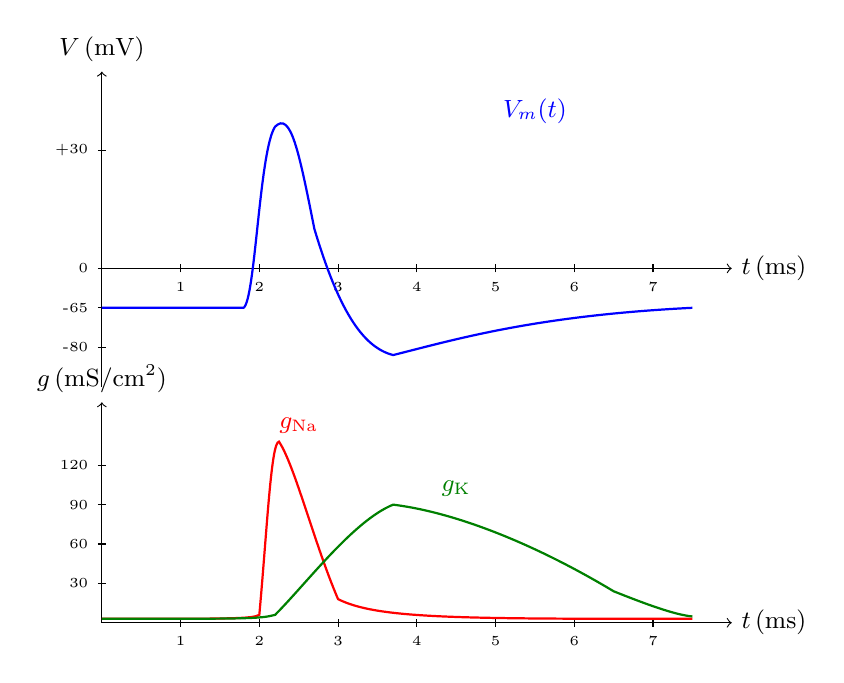
\begin{tikzpicture}[scale=1.0, every node/.style={font=\small}]
  \begin{scope}
    % Axes for voltage trace
    \draw[->] (0,0) -- (8.0,0) node[right] {$t$\,(ms)};
    \draw[->] (0,-1.5) -- (0,2.5) node[above] {$V$\,(mV)};
    % Tick marks
    \foreach \x/\t in {1/1, 2/2, 3/3, 4/4, 5/5, 6/6, 7/7} {
      \draw (\x,-0.05) -- (\x,0.05);
      \node[below] at (\x,-0.05) {\tiny \t};
    }
    \foreach \y/\t in {-1/-80, -0.5/-65, 0/0, 1.5/+30} {
      \draw (-0.05,\y) -- (0.05,\y);
      \node[left] at (-0.05,\y) {\tiny \t};
    }
    % Action potential curve (approximate piecewise)
    \draw[thick, blue] (0,-0.5)
      .. controls (1.2,-0.5) and (1.6,-0.5) .. (1.8,-0.5)
      .. controls (1.95,-0.4) and (2.0,1.5) .. (2.2,1.8)
      .. controls (2.4,2.0) and (2.5,1.5) .. (2.7,0.5)
      .. controls (3.0,-0.5) and (3.3,-1.0) .. (3.7,-1.1)
      .. controls (4.5,-0.9) and (5.5,-0.6) .. (7.5,-0.5);
    \node[align=center, color=blue] at (5.5,2.0) {$V_m(t)$};
  \end{scope}

  \begin{scope}[yshift=-4.5cm]
    % Conductance axes
    \draw[->] (0,0) -- (8.0,0) node[right] {$t$\,(ms)};
    \draw[->] (0,0) -- (0,2.8) node[above] {$g$\,(mS/cm$^2$)};
    \foreach \x/\t in {1/1, 2/2, 3/3, 4/4, 5/5, 6/6, 7/7} {
      \draw (\x,-0.05) -- (\x,0.05);
      \node[below] at (\x,-0.05) {\tiny \t};
    }
    \foreach \y/\t in {0.5/30, 1.0/60, 1.5/90, 2.0/120} {
      \draw (-0.05,\y) -- (0.05,\y);
      \node[left] at (-0.05,\y) {\tiny \t};
    }
    % Sodium conductance (sharp peak)
    \draw[thick, red] (0,0.05)
      .. controls (1.7,0.05) and (1.9,0.05) .. (2.0,0.1)
      .. controls (2.1,1.2) and (2.15,2.3) .. (2.25,2.3)
      .. controls (2.45,2.0) and (2.7,1.0) .. (3.0,0.3)
      .. controls (3.5,0.05) and (4.5,0.05) .. (7.5,0.05);
    \node[color=red] at (2.5,2.5) {$g_{\mathrm{Na}}$};
    % Potassium conductance (delayed, sustained)
    \draw[thick, color=green!50!black] (0,0.05)
      .. controls (1.9,0.05) and (2.0,0.05) .. (2.2,0.1)
      .. controls (2.6,0.5) and (3.2,1.3) .. (3.7,1.5)
      .. controls (4.5,1.4) and (5.5,1.0) .. (6.5,0.4)
      .. controls (7.0,0.2) and (7.3,0.1) .. (7.5,0.08);
    \node[color=green!50!black] at (4.5,1.7) {$g_{\mathrm{K}}$};
  \end{scope}
\end{tikzpicture}
\caption[Hodgkin-Huxley conductances during an action potential]{The
membrane potential during a single action potential (top) and the
underlying sodium and potassium conductances (bottom). Sodium
conductance rises sharply on threshold crossing, peaks within
0.5\,ms, and inactivates; potassium conductance rises with a delay
and decays slowly, repolarising the membrane. After Hodgkin and Huxley
(1952), figure adapted from squid giant axon data at $6.3\,\degC$.}
\label{fig:vol06:ch07:hh-conductances}
\end{figure}


\section{Action potentials and signal propagation}\pathtag{core}

The \engterm{action potential} is a self-propagating, all-or-nothing
voltage pulse that carries information along axons over arbitrary
distances. The mechanism was established by the Hodgkin-Huxley
work of 1952 \cite{paper:v6c07-hodgkin-huxley-1952,paper:v6c07-hodgkin-huxley-1952b},
which used the voltage-clamp technique of Cole and Marmont
\cite{paper:v6c07-cole-1949} to isolate the sodium and potassium
ionic currents. The result was awarded the Nobel Prize in 1963 and
remains the canonical example of a quantitative mechanistic model in
biology.

\engterm{The Hodgkin-Huxley model.} The classical Hodgkin-Huxley
description treats the squid giant axon membrane as a parallel
combination of three ionic currents and a capacitance:
\begin{equation}
C_m \frac{dV}{dt} = -\bar{g}_{\text{Na}} m^3 h (V - E_{\text{Na}}) - \bar{g}_K n^4 (V - E_K) - g_L (V - E_L) + I_{\text{ext}}(t).
\label{eq:hh}
\end{equation}
The maximum conductances and reversal potentials Hodgkin and Huxley
fit to their squid-axon voltage-clamp data at $6.3\,\degC$ are
$\bar{g}_{\text{Na}} = 120\,\text{mS}/\text{cm}^2$,
$\bar{g}_K = 36\,\text{mS}/\text{cm}^2$,
$g_L = 0.3\,\text{mS}/\text{cm}^2$,
$E_{\text{Na}} = +50\,\text{mV}$,
$E_K = -77\,\text{mV}$,
$E_L = -54.4\,\text{mV}$,
$C_m = 1\,\si{\micro\farad}/\text{cm}^2$
\cite[p.~520]{paper:v6c07-hodgkin-huxley-1952}.

\engterm{The gating variables.} Each of $m$, $h$, $n$ is a unitless
probability between $0$ and $1$ that the corresponding channel
``subunit'' is in the conducting configuration. The variables obey
first-order ODEs of the form
\begin{equation}
\frac{dx}{dt} = \alpha_x(V) (1 - x) - \beta_x(V) x = \frac{x_\infty(V) - x}{\tau_x(V)},
\label{eq:hh-gate}
\end{equation}
with the rate constants $\alpha_x(V), \beta_x(V)$ specific to each
gating variable. In the original parametrisation
\cite[p.~518]{paper:v6c07-hodgkin-huxley-1952}:
\begin{align*}
\alpha_m(V) &= \tfrac{0.1(V+40)}{1 - e^{-(V+40)/10}}, &
\beta_m(V) &= 4 e^{-(V+65)/18}, \\
\alpha_h(V) &= 0.07 e^{-(V+65)/20}, &
\beta_h(V) &= \tfrac{1}{1+e^{-(V+35)/10}}, \\
\alpha_n(V) &= \tfrac{0.01(V+55)}{1-e^{-(V+55)/10}}, &
\beta_n(V) &= 0.125 e^{-(V+65)/80}.
\end{align*}
The variable $m$ is the sodium-activation gate, fast and rising on
depolarisation; $h$ is the sodium-inactivation gate, slow and falling
on depolarisation; $n$ is the potassium-activation gate, slow and
rising on depolarisation. The script \verb|hodgkin_huxley.py|
integrates the system and reproduces single action potentials, the
strength-duration curve, and the repetitive firing under sustained
current.

\engterm{The mechanism in six phases.} Phase~1 (resting): the membrane
sits near $E_K$ because $g_K$ dominates ($g_K \gg g_{\text{Na}}$ at
rest). Phase~2 (depolarisation): a stimulus raises $V$ past
$\sim -55\,\text{mV}$; $m$ activates (rises) faster than $h$
inactivates (falls), and $g_{\text{Na}} = \bar{g}_{\text{Na}} m^3 h$
rises by three orders of magnitude. Phase~3 (peak): $V$ approaches
$E_{\text{Na}}$ at $+50\,\text{mV}$. Phase~4 (repolarisation): $h$
falls (sodium inactivation), $n$ rises (delayed-rectifier potassium
activation), and the membrane is driven back toward $E_K$. Phase~5
(hyperpolarisation): potassium conductance overshoots, briefly pulling
$V$ below $V_{\text{rest}}$ toward $E_K$. Phase~6 (recovery):
potassium channels close, sodium inactivation lifts, and the membrane
returns to rest. Figures~\ref{fig:vol06:ch07:hh-conductances} and
\ref{fig:vol06:ch07:ap-cycle} show the voltage and conductance time
courses; the script \verb|hodgkin_huxley.py| reproduces them.

\begin{figure}[htbp]
\centering
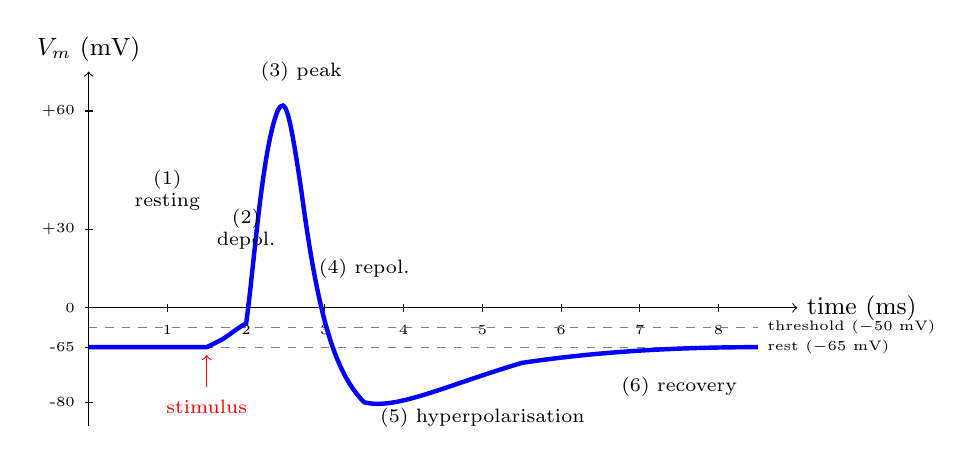
\begin{tikzpicture}[scale=1.0, every node/.style={font=\small}]
  % Axes
  \draw[->] (0,0) -- (9.0,0) node[right] {time (ms)};
  \draw[->] (0,-1.5) -- (0,3.0) node[above] {$V_m$ (mV)};
  % Tick marks x
  \foreach \x/\t in {1/1, 2/2, 3/3, 4/4, 5/5, 6/6, 7/7, 8/8} {
    \draw (\x,-0.05) -- (\x,0.05);
    \node[below] at (\x,-0.1) {\tiny \t};
  }
  % Tick marks y
  \foreach \y/\t in {-1.2/-80, -0.5/-65, 0/0, 1.0/+30, 2.5/+60} {
    \draw (-0.05,\y) -- (0.05,\y);
    \node[left] at (-0.05,\y) {\tiny \t};
  }
  % Threshold line
  \draw[dashed, color=gray] (0,-0.25) -- (8.5,-0.25);
  \node[right, font=\tiny] at (8.5,-0.25) {threshold ($-50$ mV)};
  % Resting line
  \draw[dashed, color=gray] (0,-0.5) -- (8.5,-0.5);
  \node[right, font=\tiny] at (8.5,-0.5) {rest ($-65$ mV)};
  % Action potential trace
  \draw[ultra thick, blue]
    (0,-0.5)
    .. controls (1.0,-0.5) and (1.4,-0.5) .. (1.5,-0.5)
    -- (1.7,-0.4)
    .. controls (1.85,-0.3) and (1.9,-0.25) .. (2.0,-0.2)
    .. controls (2.1,0.5) and (2.2,2.0) .. (2.4,2.5)
    .. controls (2.5,2.7) and (2.55,2.5) .. (2.7,1.5)
    .. controls (2.9,0.0) and (3.1,-0.8) .. (3.5,-1.2)
    .. controls (3.9,-1.3) and (4.5,-1.0) .. (5.5,-0.7)
    .. controls (6.5,-0.55) and (7.5,-0.5) .. (8.5,-0.5);
  % Phase annotations
  \node[align=center, font=\scriptsize] at (1.0,1.5) {(1)\\resting};
  \node[align=center, font=\scriptsize] at (2.0,1.0) {(2)\\depol.};
  \node[align=center, font=\scriptsize] at (2.7,3.0) {(3) peak};
  \node[align=center, font=\scriptsize] at (3.5,0.5) {(4) repol.};
  \node[align=center, font=\scriptsize] at (5.0,-1.4) {(5) hyperpolarisation};
  \node[align=center, font=\scriptsize] at (7.5,-1.0) {(6) recovery};
  % Stimulus arrow
  \draw[->, color=red] (1.5,-1.0) -- (1.5,-0.6);
  \node[below, color=red, font=\scriptsize] at (1.5,-1.05) {stimulus};
\end{tikzpicture}
\caption[Action potential cycle]{The six phases of the action potential:
(1)~resting at $-65\,\text{mV}$ with closed voltage-gated channels;
(2)~depolarisation as voltage-gated sodium channels open;
(3)~peak near $+30\,\text{mV}$;
(4)~repolarisation as sodium channels inactivate and potassium channels
open; (5)~hyperpolarisation overshoot below resting; (6)~recovery to
rest as potassium channels close. The absolute refractory period
spans phases (3) through early (4); the relative refractory period
extends through (5) and (6).}
\label{fig:vol06:ch07:ap-cycle}
\end{figure}


\engterm{The refractory periods.} The absolute refractory period
($\sim 1$ to $2\,\text{ms}$) is set by sodium-channel inactivation:
while $h$ is small, no stimulus can produce another action potential,
because the available sodium conductance is too low. The relative
refractory period ($\sim 5$ to $10\,\text{ms}$) follows: once $h$
recovers, action potentials can fire but at higher threshold because
the delayed-rectifier potassium current is still elevated. Refractory
behaviour sets the maximum sustainable firing rate at roughly
$500$ to $1000\,\text{Hz}$ for the fastest neurons and $\sim 100\,\text{Hz}$
for typical cortical pyramidal cells (Table at
\verb|data/firing_rates_by_cell_type.csv|).

\engterm{Propagation.} An action potential at one location depolarises
the adjacent membrane through axial current spread, and (if the
adjacent region's threshold is crossed) triggers an action potential
there, propagating the pulse along the axon. The propagation velocity
in unmyelinated axons scales as $\sqrt{d}$ where $d$ is the axon
diameter, derived from cable theory by equating the axial-current
charge-up time to the action-potential rise time. In myelinated axons
the velocity scales linearly with $d$ due to saltatory conduction:
the axon is wrapped in oligodendrocyte- or Schwann-cell-derived myelin
that acts as an insulator over $1$ to $2\,\text{mm}$ stretches between
unmyelinated nodes of Ranvier ($\sim 1\,\si{\micro\meter}$ long); the
action potential regenerates only at the nodes and ``jumps'' between
them through the high-resistance myelinated internode. Velocities
range from $1\,\text{m}/\text{s}$ in small unmyelinated C fibres
(carrying slow pain and temperature) to $120\,\text{m}/\text{s}$ in
the largest myelinated A$\alpha$ motor fibres
\cite[ch.~6]{text:v6c07-kandel-principles-2021}. The diameter and
myelination of an axon are evolutionary engineering choices: large
myelinated axons are fast but expensive in volume and energy; small
unmyelinated axons are cheap but slow.

\engterm{The metabolic cost.} Each action potential requires ATP to
restore the ionic gradients. The sodium that entered must be pumped
back out by the Na/K-ATPase, which exchanges $3$ Na$^+$ for $2$ K$^+$
per ATP. The energy cost per action potential is approximately
$5 \times 10^8\,\text{ATP}$ per cm of axon length in mammalian
neurons; integrated over the brain's neuronal population, the action
potentials, postsynaptic currents, and resting potential maintenance
together consume approximately $20\,\%$ of the body's resting
metabolic rate \cite{paper:v6c07-attwell-laughlin-2001}. The high
cost is the engineering trade-off for the action potential's speed
and reliability.

\begin{principle}[The action potential is digital signalling in a noisy analog substrate]
The neuron converts analog membrane-potential inputs (the
sub-threshold synaptic potentials) into digital output spikes through
the action-potential mechanism. The conversion is robust to noise:
brief spurious depolarisations below threshold do not propagate;
sustained suprathreshold depolarisations produce reliable spike
trains. The spike rate (and, in some systems, the spike timing
relative to a population reference) carries the information; the
spike shape carries none. The architecture is a noise-resistant
digital encoding in a chemically and thermally noisy analog substrate,
and is one of the clearest examples in biology of a robust engineering
solution to a signal-to-noise problem.
\end{principle}

\section{Synapses and networks}\pathtag{standard}

A neuron communicates with other neurons through synapses, the
junction points at which an axon terminal of one neuron contacts a
dendrite or soma of another. The synapse converts the electrical
signal of the presynaptic action potential into a chemical signal
(neurotransmitter release) and back into an electrical signal
(postsynaptic potential change), with a delay of $\sim 0.5\,\text{ms}$
and the option to amplify, attenuate, or invert the signal in passing.

\begin{figure}[htbp]
\centering
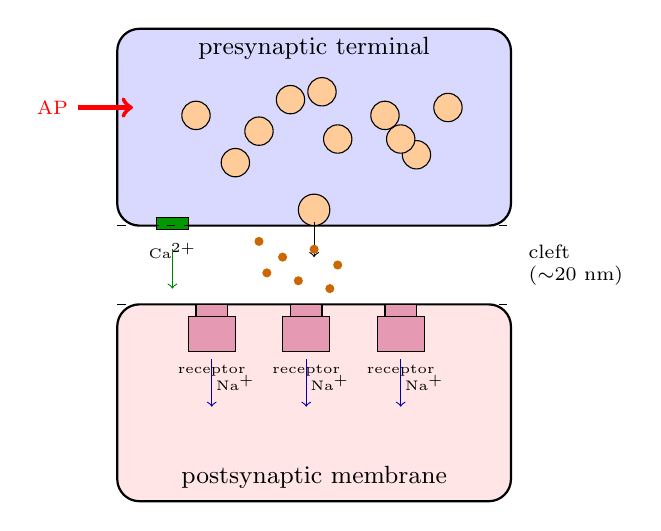
\begin{tikzpicture}[scale=1.0, every node/.style={font=\small}]
  % Presynaptic terminal
  \draw[thick, fill=blue!15, rounded corners=8pt] (0,2) rectangle (5,4.5);
  \node at (2.5,4.25) {presynaptic terminal};
  % Vesicles in presynaptic
  \foreach \x/\y in {1.0/3.4, 1.5/2.8, 2.2/3.6, 2.8/3.1, 3.4/3.4, 3.8/2.9, 4.2/3.5, 1.8/3.2, 2.6/3.7, 3.6/3.1} {
    \draw[fill=orange!40] (\x,\y) circle (0.18);
  }
  % Vesicle fusing
  \draw[fill=orange!40] (2.5,2.2) circle (0.2);
  \draw[->] (2.5,2.05) -- (2.5,1.6);
  % Action potential arrow
  \draw[->, ultra thick, color=red] (-0.5,3.5) -- (0.2,3.5);
  \node[left, color=red, font=\scriptsize] at (-0.5,3.5) {AP};
  % Voltage-gated Ca channel
  \draw[fill=green!60!black] (0.5,1.95) rectangle (0.9,2.1);
  \node[below, font=\tiny] at (0.7,1.9) {Ca$^{2+}$};
  \draw[->, color=green!50!black] (0.7,1.7) -- (0.7,1.2);
  % Synaptic cleft
  \draw[dashed] (0,2) -- (5,2);
  \draw[dashed] (0,1.0) -- (5,1.0);
  \node[right, align=left, font=\scriptsize] at (5.1,1.5) {cleft\\($\sim$20 nm)};
  % Neurotransmitter dots in cleft
  \foreach \x/\y in {1.8/1.8, 2.1/1.6, 2.5/1.7, 2.8/1.5, 2.3/1.3, 2.7/1.2, 1.9/1.4} {
    \filldraw[orange!80!black] (\x,\y) circle (0.05);
  }
  % Postsynaptic membrane
  \draw[thick, fill=red!10, rounded corners=8pt] (0,-1.5) rectangle (5,1.0);
  \node at (2.5,-1.2) {postsynaptic membrane};
  % Receptors
  \foreach \x in {1.2, 2.4, 3.6} {
    \draw[fill=purple!40] (\x-0.2,0.85) rectangle (\x+0.2,1.0);
    \draw[fill=purple!40] (\x-0.3,0.4) rectangle (\x+0.3,0.85);
    \node[below, font=\tiny] at (\x,0.35) {receptor};
  }
  % Ion influx arrows
  \foreach \x in {1.2, 2.4, 3.6} {
    \draw[->, color=blue!70!black] (\x,0.3) -- (\x,-0.3);
    \node[font=\tiny] at (\x+0.3,0.0) {Na$^+$};
  }
\end{tikzpicture}
\caption[Chemical synapse]{A chemical synapse. An incoming action
potential opens voltage-gated calcium channels at the presynaptic
terminal; calcium influx triggers vesicle fusion; neurotransmitter
diffuses across the $\sim 20\,\text{nm}$ cleft in $\sim 0.05\,\text{ms}$
and binds postsynaptic ligand-gated receptors that open ion-selective
channels and change the postsynaptic membrane potential.}
\label{fig:vol06:ch07:synapse}
\end{figure}


\engterm{Chemical synapses.} The standard chemical synapse comprises
a presynaptic terminal (containing $\sim 100$ to $10\,000$ vesicles
full of neurotransmitter), a synaptic cleft ($\sim 20\,\text{nm}$
wide), and a postsynaptic membrane (with neurotransmitter receptors
clustered into a postsynaptic density). When an action potential
arrives at the presynaptic terminal, voltage-gated calcium channels
open, calcium enters the terminal, and the calcium triggers the fusion
of vesicles with the presynaptic membrane through the SNARE
complex, releasing the neurotransmitter into the cleft. The
neurotransmitter diffuses across the cleft (transit time
$\sim 0.05\,\text{ms}$) and binds receptors on the postsynaptic
membrane, producing a brief change in postsynaptic conductance and
hence in postsynaptic membrane potential. The full sequence
(arrival of action potential, calcium influx, vesicle fusion,
diffusion, receptor binding, channel opening) takes about
$0.5\,\text{ms}$, the synaptic delay.

\engterm{Quantal release.} Bernard Katz and colleagues showed in the
1950s that neurotransmitter release is quantal: the postsynaptic
response is built from integer multiples of a unit response,
corresponding to the release of one vesicle. A typical vesicle
contains $\sim 5000$ molecules of transmitter; a typical presynaptic
action potential releases $\sim 1$ to $10$ vesicles, with the release
probability per vesicle ranging from $0.1$ to $0.9$ across synapse
types. The statistics are well-described by binomial distributions
with refinements for facilitation, depression, and asynchronous
release \cite[ch.~12]{text:v6c07-kandel-principles-2021}.

\engterm{Synaptic timescales.} The full transmitter-receptor cycle
spans several disparate timescales. Calcium influx peaks within
$0.2\,\text{ms}$ of the presynaptic action potential. Vesicle fusion
takes $0.1$ to $0.5\,\text{ms}$. Transmitter diffusion across the
cleft takes $\sim 0.05\,\text{ms}$. Postsynaptic channel opening
(AMPA-type glutamate receptors) takes $\sim 0.1\,\text{ms}$; the
channels then close with a time constant of $\sim 1$ to $5\,\text{ms}$,
producing the excitatory postsynaptic current (EPSC). NMDA-type
glutamate receptors open more slowly ($\sim 5\,\text{ms}$) and stay
open longer ($\sim 100\,\text{ms}$), giving them a special role in
coincidence detection and in long-term plasticity. GABA$_A$ receptors
open in $\sim 1\,\text{ms}$ and stay open for $\sim 10\,\text{ms}$,
producing inhibitory postsynaptic currents. Metabotropic receptors
act through G-protein cascades on timescales of $100\,\text{ms}$ to
seconds. The script \verb|synaptic_dynamics.py| illustrates the
alpha-function approximation $g(t) = g_{\text{peak}} (t/\tau)
e^{1-t/\tau}$ to the EPSC waveform.

\engterm{Neurotransmitters.} The principal mammalian neurotransmitters
are: \engterm{glutamate} (the dominant excitatory transmitter in the
central nervous system), \engterm{GABA} (the dominant inhibitory
transmitter in the central nervous system), \engterm{acetylcholine}
(at the neuromuscular junction and in cholinergic central pathways),
\engterm{dopamine} (reward and motor pathways), \engterm{serotonin}
(mood and arousal), and \engterm{noradrenaline} (autonomic and
arousal). Each transmitter has multiple receptor subtypes with
different signalling properties; the same transmitter can be
excitatory at one synapse and inhibitory at another depending on the
receptor and on the intracellular chloride concentration of the
postsynaptic cell.

\engterm{Short-term plasticity.} Synaptic strength varies on a per-
spike basis. \engterm{Facilitation} (presynaptic calcium accumulation
boosting release probability) and \engterm{depression} (vesicle
depletion limiting release) operate on timescales of $50$ to
$500\,\text{ms}$. The Tsodyks-Markram model
\cite{paper:v6c07-tsodyks-markram-1997} formalises both as a pair of
ODEs for the available-resource fraction $R$ and the
release-probability factor $u$ that the synaptic-dynamics script
reproduces.

\engterm{Long-term plasticity.} \engterm{Long-term potentiation} (LTP),
discovered by Bliss and L\o mo in 1973 in the rabbit hippocampus
\cite{paper:v6c07-bliss-lomo-1973}, is a long-lasting increase in
synaptic strength following high-frequency stimulation;
\engterm{long-term depression} (LTD) is a long-lasting decrease
following low-frequency stimulation. Both are mediated by changes in
the number, distribution, and phosphorylation of postsynaptic AMPA
receptors, triggered downstream of calcium influx through NMDA
receptors. The Hebbian summary (neurons that fire together wire
together; Hebb 1949 \cite{text:v6c07-hebb-1949}) captures the broad
outline; the detailed molecular machinery occupies a substantial
literature \cite[chs.~66--67]{text:v6c07-kandel-principles-2021}. LTP
is the cellular basis of associative learning and memory.

\engterm{Networks.} The human brain contains $\sim 8.6 \times 10^{10}$
neurons \cite[ch.~1]{text:v6c07-kandel-principles-2021}, each with
$10^3$ to $10^4$ synaptic connections, for a total of $\sim 10^{14}$
to $10^{15}$ synapses. The brain is organised hierarchically (sensory
cortices, association areas, motor cortices) with extensive recurrent
and feedback connectivity. The functional organisation has been mapped
at multiple scales: cytoarchitectonic regions, functional areas
defined by lesion studies and functional imaging, columnar
microcircuits about $0.5\,\text{mm}$ across. A reader who wishes to
enter neuroscience seriously should consult Kandel
\cite{text:v6c07-kandel-principles-2021} for the architectural
detail; the engineering reading developed here is sufficient for
control-systems applications.

\section{The nervous system as distributed control}\pathtag{core}

The nervous system controls movement, perception, autonomic
regulation, and cognition through a distributed control architecture
that the engineer can read as a multi-layered control system with
sensors, effectors, and integration at every level
(Figure~\ref{fig:vol06:ch07:ns-hierarchy}).

\begin{figure}[htbp]
\centering
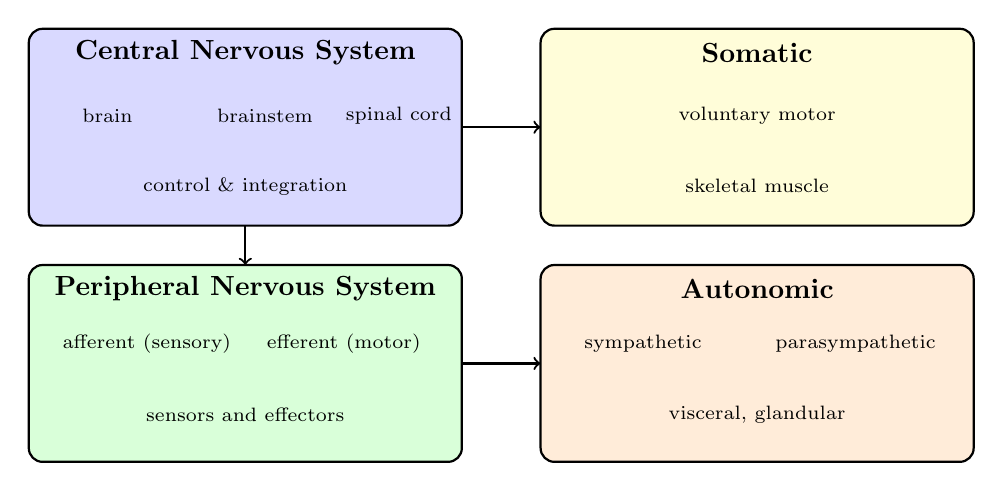
\begin{tikzpicture}[scale=1.0, every node/.style={font=\small}]
  % CNS box
  \draw[thick, fill=blue!15, rounded corners=5pt] (0,3) rectangle (5.5,5.5);
  \node[font=\bfseries] at (2.75,5.2) {Central Nervous System};
  \node[align=center, font=\scriptsize] at (1.0,4.4) {brain};
  \node[align=center, font=\scriptsize] at (3.0,4.4) {brainstem};
  \node[align=center, font=\scriptsize] at (4.7,4.4) {spinal cord};
  \node[align=center, font=\scriptsize] at (2.75,3.5) {control \& integration};
  % PNS box
  \draw[thick, fill=green!15, rounded corners=5pt] (0,0) rectangle (5.5,2.5);
  \node[font=\bfseries] at (2.75,2.2) {Peripheral Nervous System};
  \node[align=center, font=\scriptsize] at (1.5,1.5) {afferent (sensory)};
  \node[align=center, font=\scriptsize] at (4.0,1.5) {efferent (motor)};
  \node[align=center, font=\scriptsize] at (2.75,0.6) {sensors and effectors};
  % Autonomic box
  \draw[thick, fill=orange!15, rounded corners=5pt] (6.5,0) rectangle (12,2.5);
  \node[font=\bfseries] at (9.25,2.2) {Autonomic};
  \node[align=center, font=\scriptsize] at (7.8,1.5) {sympathetic};
  \node[align=center, font=\scriptsize] at (10.5,1.5) {parasympathetic};
  \node[align=center, font=\scriptsize] at (9.25,0.6) {visceral, glandular};
  % Somatic label
  \draw[thick, fill=yellow!15, rounded corners=5pt] (6.5,3) rectangle (12,5.5);
  \node[font=\bfseries] at (9.25,5.2) {Somatic};
  \node[align=center, font=\scriptsize] at (9.25,4.4) {voluntary motor};
  \node[align=center, font=\scriptsize] at (9.25,3.5) {skeletal muscle};
  % Arrows
  \draw[->, thick] (2.75,3) -- (2.75,2.5);
  \draw[->, thick] (5.5,1.25) -- (6.5,1.25);
  \draw[->, thick] (5.5,4.25) -- (6.5,4.25);
\end{tikzpicture}
\caption[Nervous system hierarchy]{The vertebrate nervous system at a
glance. The central nervous system (brain and spinal cord) integrates
sensory input and issues motor commands. The peripheral nervous system
carries information between the CNS and the body, with somatic
(voluntary) and autonomic (involuntary) branches; the autonomic
divides into sympathetic and parasympathetic arms.}
\label{fig:vol06:ch07:ns-hierarchy}
\end{figure}


\engterm{The central nervous system.} The brain and spinal cord
constitute the central nervous system (CNS). The brain has four
principal subdivisions. The brainstem regulates vital functions
(breathing, cardiovascular control). The cerebellum coordinates
movement and timing. The diencephalon (thalamus and hypothalamus)
relays sensory input and controls autonomic and endocrine output.
The cerebrum (cortex and basal ganglia) handles sensorimotor,
cognitive, and limbic functions. Each subdivision contributes
distinct control functions; lesions to each produce characteristic
deficits, which is how the functional map was originally established.

\engterm{The peripheral nervous system.} The peripheral nervous
system carries information between the CNS and the body. Afferent
fibres carry sensory information toward the CNS; efferent fibres
carry motor and autonomic commands away from the CNS. The motor
system divides into the somatic (controlling skeletal muscle) and
the autonomic (controlling smooth muscle, cardiac muscle, and
glands). The autonomic divides into the sympathetic (fight-or-flight
responses, mediated mainly by noradrenaline) and the parasympathetic
(rest-and-digest responses, mediated mainly by acetylcholine).

\engterm{Motor control.} The execution of voluntary movement involves
a hierarchical control architecture: the motor cortex selects the
movement; the basal ganglia and cerebellum modify the selection in
response to context and feedback; the brainstem and spinal cord
generate the motor patterns; the muscles execute. Feedback is
provided by proprioceptive receptors (muscle spindles, Golgi tendon
organs) and visual and vestibular inputs. The whole control loop
operates with a delay of $\sim 50$ to $200\,\text{ms}$, which sets
the timescale on which voluntary movements can be corrected by
feedback. Fast corrections are handled by lower control layers
(reflexes); slow corrections involve cortical processing.

\engterm{Reflex arcs.} The simplest motor control is the spinal reflex:
a sensory input (e.g.\ muscle stretch) directly activates a motor
output (muscle contraction) through a small number of synapses in the
spinal cord, with no involvement of the brain. The patellar
(knee-jerk) reflex is the textbook example: a tap on the patellar
tendon stretches the quadriceps muscle, which activates muscle-spindle
sensory fibres, which monosynaptically excite the quadriceps motor
neurons in the spinal cord, which produce the knee extension. The
reflex latency is $\sim 30\,\text{ms}$, far faster than any
voluntary response. Spinal reflexes are the lowest-level controllers
in the motor hierarchy.

\engterm{Sensory transduction.} Sensory receptors convert physical
stimuli into electrical signals. The principal modalities are
mechanical (touch, proprioception, hearing), chemical (taste, smell),
thermal (warmth, cold), photic (vision), and nociceptive (pain). Each
receptor type has a specific transduction mechanism: hair cells in
the ear use mechanoelectric transduction at the apical tip-link;
photoreceptors in the retina use a G-protein-coupled cascade triggered
by photoisomerisation of rhodopsin; olfactory neurons use
G-protein-coupled receptors of $\sim 400$ types in humans, encoding
the chemical identity of an odorant in the combinatorial activation
pattern across receptor types.

\engterm{The Bayesian-brain framing.} A productive engineering
framing reads the nervous system as a Bayesian inference machine
\cite{paper:v6c07-knill-pouget-2004}. The brain receives noisy,
ambiguous sensory data and must infer the underlying state of the
world. Under the framing, neural populations represent probability
distributions; integration of multiple cues corresponds to Bayes'
rule; decision-making corresponds to posterior sampling or maximum-a-
posteriori estimation. Karl Friston's free-energy principle
\cite{paper:v6c07-friston-2010} extends the framing to action: the
brain selects actions that minimise the expected divergence between
its predictions and incoming sensory data, equivalent (under
appropriate assumptions) to maximising the model evidence for its
internal generative model. The framing is mathematically clean and
empirically productive; whether it is the correct framing for all
neural computation remains an open question in the literature.

\begin{archetype}[Control and interface in biological signalling]
The nervous system exhibits the control archetype in its most
quantitative biological form. The action potential is a digital
encoding; the synapse is an adjustable gain element with short- and
long-term dynamics; the network of neurons implements a control
architecture with sensing, computation, and actuation across multiple
hierarchical layers. The interface archetype appears at every level:
at the synapse between neurons, at the neuromuscular junction between
nervous system and muscle, at the sensory receptors between body and
world, at the blood-brain barrier between vascular and neural
compartments. The immune system, developed in the next sections,
exhibits the same archetypes at a different timescale (hours to weeks
rather than milliseconds) and in a different physical domain
(molecular recognition rather than electrical signalling).
\end{archetype}

\section{The immune system: recognition, response, memory}\pathtag{standard}

The immune system is the body's distributed defence against
pathogens and against cellular abnormalities (cancer, damaged cells).
The system has three principal functions, organised in time:
\engterm{recognition} of foreign or aberrant material;
\engterm{response} that eliminates the recognised threat; and
\engterm{memory} that accelerates the response to subsequent
encounters with the same threat. Figure~\ref{fig:vol06:ch07:immune-timeline}
shows the characteristic timelines of the innate and adaptive arms.

\begin{figure}[htbp]
\centering
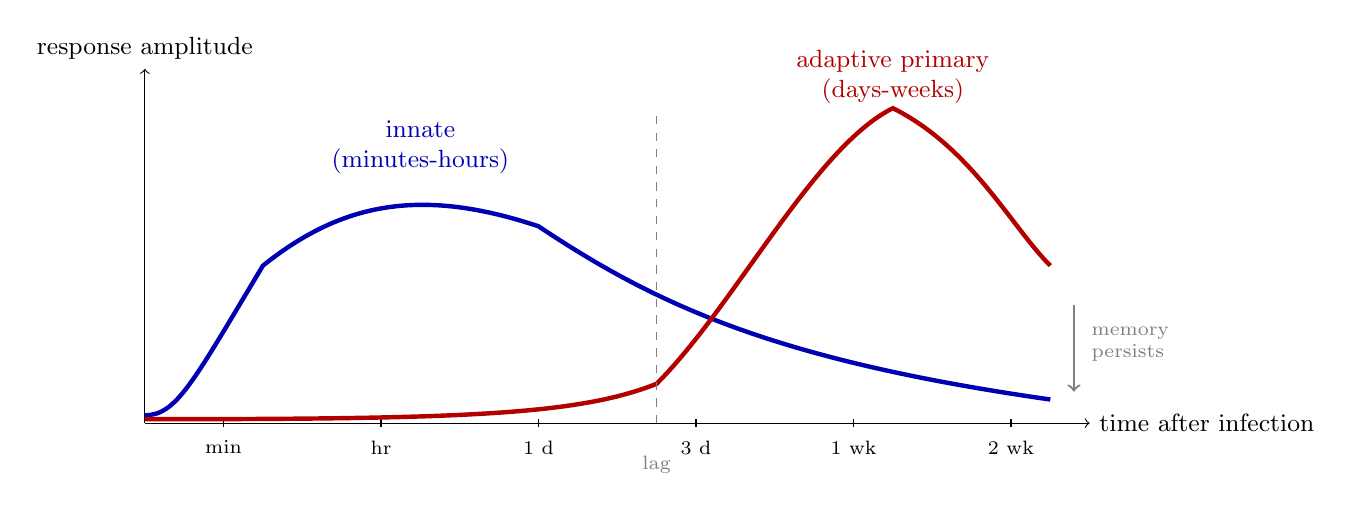
\begin{tikzpicture}[scale=1.0, every node/.style={font=\small}]
  % Axes
  \draw[->] (0,0) -- (12.0,0) node[right] {time after infection};
  \draw[->] (0,0) -- (0,4.5) node[above] {response amplitude};
  % Time tick marks
  \foreach \x/\t in {1/min, 3/hr, 5/1 d, 7/3 d, 9/1 wk, 11/2 wk} {
    \draw (\x,-0.05) -- (\x,0.05);
    \node[below, font=\scriptsize] at (\x,-0.1) {\t};
  }
  % Innate response curve (fast rise, modest peak, falls)
  \draw[ultra thick, color=blue!70!black]
    (0,0.1) .. controls (0.4,0.1) and (0.6,0.5) ..
    (1.5,2.0) .. controls (2.5,2.8) and (3.5,3.0) ..
    (5.0,2.5) .. controls (6.5,1.5) and (8.0,0.8) ..
    (11.5,0.3);
  \node[color=blue!70!black, align=center] at (3.5,3.5) {innate\\(minutes-hours)};
  % Adaptive primary response (slow rise, large peak, slow fall)
  \draw[ultra thick, color=red!70!black]
    (0,0.05) .. controls (4.0,0.05) and (5.5,0.1) ..
    (6.5,0.5) .. controls (7.5,1.5) and (8.5,3.5) ..
    (9.5,4.0) .. controls (10.5,3.5) and (11.0,2.5) ..
    (11.5,2.0);
  \node[color=red!70!black, align=center] at (9.5,4.4) {adaptive primary\\(days-weeks)};
  % Dashed line marking onset of adaptive
  \draw[dashed, gray] (6.5,0) -- (6.5,4.0);
  \node[below, font=\scriptsize, color=gray] at (6.5,-0.3) {lag};
  % Memory phase indication
  \draw[->, thick, gray] (11.8,1.5) -- (11.8,0.4);
  \node[right, font=\scriptsize, color=gray, align=left] at (11.9,1.0) {memory\\persists};
\end{tikzpicture}
\caption[Innate and adaptive immune response timelines]{Time courses
of the innate (blue) and adaptive (red) immune responses to a primary
infection. The innate response activates within minutes and peaks
within hours; the adaptive primary response lags by days, peaks at
day 10 to 14, and falls slowly, leaving a memory population that
mounts a faster and larger response on re-encounter.}
\label{fig:vol06:ch07:immune-timeline}
\end{figure}


\engterm{Cellular components.} The immune system uses several distinct
cell types. \engterm{Innate immune cells} (neutrophils, macrophages,
natural killer cells, dendritic cells) respond rapidly and
non-specifically to pathogen-associated molecular patterns.
\engterm{Adaptive immune cells} (T lymphocytes and B lymphocytes)
respond more slowly but with antigen-specific receptors that
discriminate among millions of distinct molecular targets.
\engterm{Antigen-presenting cells} (dendritic cells, macrophages,
B cells) capture antigens and display them to T cells, bridging the
innate and adaptive arms of the response. The total leukocyte
population in adult human blood is $\sim 4 \times 10^9$ cells per
litre, distributed across the principal types in well-characterised
ratios \cite[ch.~1]{text:v6c07-janeway-immunobiology-2017}.

\engterm{Lymphoid organs.} The immune system is housed in lymphoid
tissues distributed throughout the body. \engterm{Primary lymphoid
organs} (bone marrow and thymus) produce immune cells.
\engterm{Secondary lymphoid organs} (lymph nodes, spleen, Peyer's
patches in the intestine, tonsils) are sites where antigens are
concentrated and where lymphocytes encounter them. The lymphatic
system, a network of vessels paralleling the blood vasculature,
carries fluid and immune cells between tissues and lymph nodes. The
architecture exposes every antigen in the body to enough lymphocytes
that some will recognise it. With $10^{12}$ to $10^{13}$ lymphocytes
in the adult human body and an antigen receptor repertoire of
$\sim 10^7$ to $10^8$ distinct specificities, the matching
probability is adequate for fast antigen detection.

\engterm{Innate recognition.} The innate immune system recognises
conserved molecular patterns associated with pathogens: bacterial
lipopolysaccharide, bacterial flagellin, viral double-stranded RNA,
fungal cell-wall components. The recognition uses germline-encoded
\engterm{pattern-recognition receptors} (Toll-like receptors,
NOD-like receptors, RIG-I-like receptors) that bind these conserved
molecules and trigger inflammatory signalling. The identification of
the first human Toll-like receptor (TLR4) by Medzhitov, Preston-
Hurlburt and Janeway in 1997 \cite{paper:v6c07-medzhitov-1997}
opened the molecular study of innate recognition. Innate recognition
is fast (minutes), reliable (the targets do not vary much across
pathogen species), but non-specific (any pathogen of a broad class is
recognised the same way).

\engterm{Adaptive recognition and clonal selection.} The adaptive
immune system uses clonally expressed antigen receptors with
somatically generated diversity. Each B cell expresses a single
membrane-bound immunoglobulin that recognises a specific antigen;
each T cell expresses a single T-cell receptor that recognises a
specific peptide-MHC complex. The receptor diversity is generated by
combinatorial V(D)J gene segment rearrangement during lymphocyte
development, demonstrated molecularly by Tonegawa in 1976--1978
\cite{paper:v6c07-tonegawa-1983} (Nobel Prize 1987). The arithmetic
of V(D)J recombination is approximately
\begin{equation}
N_{\text{TCR}} \approx N_V \times N_D \times N_J \times N_{V'} \times N_{J'} \times f_{\text{junctional}},
\label{eq:tcr-diversity}
\end{equation}
where the factors are the number of variable, diversity, and joining
segments on each chain, multiplied by the junctional-diversity factor
from non-templated nucleotide addition at the joining sites. The
total combinatorial space is $\sim 10^{15}$ to $10^{18}$ possible
TCRs; the realised repertoire in a single adult is $\sim 10^7$ to
$10^8$, sampled by stochastic gene rearrangement during thymic
development. Only the small fraction of receptors that encounter
their cognate antigen are selected for expansion (\engterm{clonal
selection}, due to Burnet in 1957
\cite{paper:v6c07-burnet-clonal-1957,text:v6c07-burnet-clonal-book-1959});
the rest die without proliferating. The result is an antigen-specific
response: only those clones with receptors that match the encountered
antigen mount a response, and the response is precisely targeted to
the encountered antigen.

\engterm{The MHC and antigen presentation.} T-cell receptors do not
recognise free antigens. They recognise short peptide fragments
displayed on cell surfaces by the major histocompatibility complex
(MHC), discovered as a histocompatibility genetic locus by George
Snell in his 1948 work on congenic mouse strains
\cite{paper:v6c07-snell-mhc-1948}. The structural basis (an open
peptide-binding groove formed by two $\alpha$-helices over a
$\beta$-sheet floor) was established crystallographically by
Bjorkman and colleagues in 1987 \cite{paper:v6c07-bjorkman-1987}. Two
classes of MHC molecule exist
(Figure~\ref{fig:vol06:ch07:mhc}):

\begin{itemize}
\item \engterm{MHC class I.} Expressed on all nucleated cells.
Displays peptides ($8$ to $10$ residues) derived from endogenously
synthesised proteins, processed in the cytosol by the proteasome and
loaded onto MHC I in the endoplasmic reticulum. Recognised by
CD8$^+$ cytotoxic T cells. Function: report on the cell's internal
state; if the cell is producing viral or aberrant proteins, the
displayed peptides will betray that, and the cytotoxic T cell will
kill the cell.

\item \engterm{MHC class II.} Restricted to professional
antigen-presenting cells (dendritic cells, macrophages, B cells).
Displays peptides ($12$ to $25$ residues) derived from extracellular
proteins taken up by endocytosis and processed in the endolysosomal
pathway. Recognised by CD4$^+$ helper T cells. Function: report on
the extracellular antigenic environment; if the APC has taken up a
pathogen, the displayed peptides will trigger help for the appropriate
B-cell and cytotoxic responses.
\end{itemize}

The discovery by Zinkernagel and Doherty in 1974
\cite{paper:v6c07-zinkernagel-doherty-1974} that T cells recognise
antigens \emph{only in the context of a specific MHC allele} (``MHC
restriction'') was awarded the 1996 Nobel Prize and remains a central
organising fact of cellular immunology. The
\verb|data/mhc_binding_affinity.csv| file collects illustrative
binding affinities for HLA-A*02:01 (a common class I allele) and
HLA-DRB1*04:01 (a common class II allele).

\engterm{Effector functions.} Once activated, immune cells eliminate
their targets through several mechanisms. Antibodies (secreted by
plasma cells, the differentiated form of activated B cells) bind to
extracellular targets and neutralise them, mark them for destruction
by complement or phagocytes, and prevent them from binding their
intended receptors on host cells (Figure~\ref{fig:vol06:ch07:antibody}).
Cytotoxic T cells recognise infected or aberrant host cells presenting
foreign peptides on MHC class I molecules and kill them by inducing
apoptosis through perforin and granzyme delivery or through Fas-Fas
ligand engagement. Helper T cells secrete cytokines that coordinate
the activities of other immune cells (Th1 cells secrete IFN-$\gamma$
to drive cellular immunity; Th2 cells secrete IL-4 and IL-13 to drive
antibody production; Th17 cells secrete IL-17 to drive neutrophil
recruitment). Phagocytes (macrophages, neutrophils, dendritic cells)
engulf and degrade extracellular targets.

\begin{figure}[htbp]
\centering
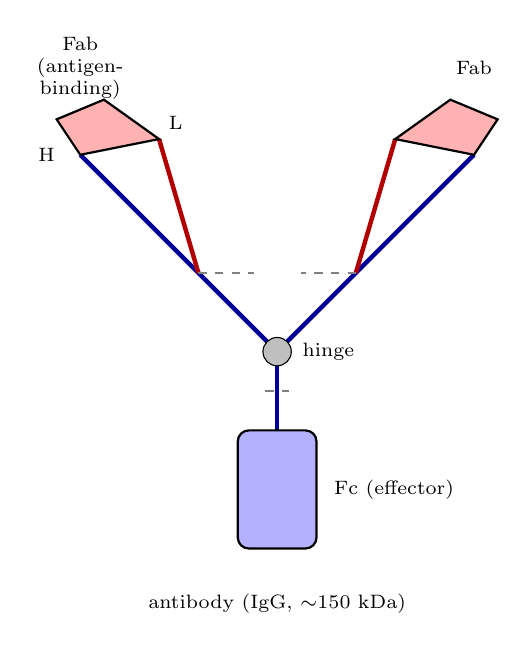
\begin{tikzpicture}[scale=1.0, every node/.style={font=\small}]
  % Heavy chains
  \draw[ultra thick, blue!60!black] (-2.5,2.5) -- (0,0) -- (2.5,2.5);
  \draw[ultra thick, blue!60!black] (0,0) -- (0,-2.5);
  % Light chains
  \draw[ultra thick, red!70!black] (-1.5,2.7) -- (-1.0,1.0);
  \draw[ultra thick, red!70!black] (1.5,2.7) -- (1.0,1.0);
  % Variable regions (Fab tips)
  \draw[fill=red!30, thick] (-2.5,2.5) -- (-2.8,2.95) -- (-2.2,3.2) -- (-1.5,2.7) -- cycle;
  \draw[fill=red!30, thick] (2.5,2.5) -- (2.8,2.95) -- (2.2,3.2) -- (1.5,2.7) -- cycle;
  % Fab labels
  \node[align=center, font=\scriptsize] at (-2.5,3.6) {Fab\\(antigen-\\binding)};
  \node[align=center, font=\scriptsize] at (2.5,3.6) {Fab};
  % Fc region
  \draw[fill=blue!30, thick, rounded corners=4pt] (-0.5,-2.5) rectangle (0.5,-1.0);
  \node[right, font=\scriptsize] at (0.6,-1.75) {Fc (effector)};
  % Hinge
  \draw[fill=gray!50] (0,0) circle (0.18);
  \node[right, font=\scriptsize] at (0.2,0) {hinge};
  % Disulfide bonds
  \draw[thick, gray, dashed] (-1.0,1.0) -- (-0.3,1.0);
  \draw[thick, gray, dashed] (1.0,1.0) -- (0.3,1.0);
  \draw[thick, gray, dashed] (-0.15,-0.5) -- (0.15,-0.5);
  % Chain labels
  \node[left, font=\scriptsize] at (-2.7,2.5) {H};
  \node[right, font=\scriptsize] at (-1.5,2.9) {L};
  % Annotation
  \node[align=center, font=\scriptsize] at (0,-3.2) {antibody (IgG, $\sim$150 kDa)};
\end{tikzpicture}
\caption[Antibody structure]{Schematic Y-shaped structure of an IgG
antibody. Two identical heavy chains (blue) and two identical light
chains (red) form a hinged structure. The Fab arms carry the
variable-region antigen-binding sites generated by somatic V(D)J
recombination; the Fc stem mediates effector functions
(complement activation, binding to Fc receptors on phagocytes and
mast cells).}
\label{fig:vol06:ch07:antibody}
\end{figure}


\engterm{Memory.} After an immune response, a small population of
\engterm{memory cells} persists for years to decades. The memory
cells respond more rapidly and more strongly to a subsequent
encounter with the same antigen, providing the long-term protection
that constitutes adaptive immunity. The memory population is the
engineering basis of vaccination: a vaccine introduces an antigen
without the pathogenic potential of the live infection and
establishes a memory population that protects against subsequent
encounters with the pathogen
\cite[ch.~11]{text:v6c07-janeway-immunobiology-2017}.

\begin{figure}[htbp]
\centering
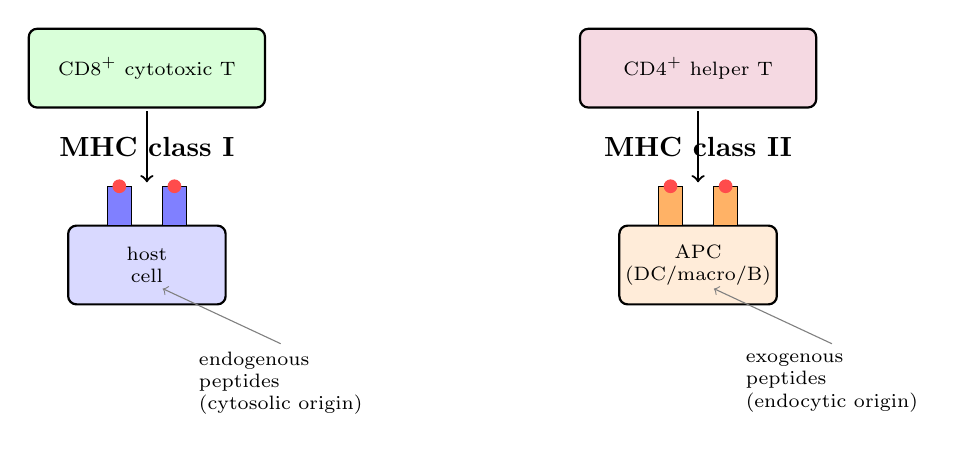
\begin{tikzpicture}[scale=1.0, every node/.style={font=\small}]
  % MHC class I panel
  \begin{scope}
    \node[font=\bfseries] at (2.5,4.5) {MHC class I};
    \draw[thick, fill=blue!15, rounded corners=3pt] (1.5,2.5) rectangle (3.5,3.5);
    \node[align=center, font=\scriptsize] at (2.5,3.0) {host\\cell};
    % MHC I on surface
    \draw[fill=blue!50] (2.0,3.5) -- (2.0,4.0) -- (2.3,4.0) -- (2.3,3.5) -- cycle;
    \draw[fill=blue!50] (2.7,3.5) -- (2.7,4.0) -- (3.0,4.0) -- (3.0,3.5) -- cycle;
    % Peptide on MHC I
    \filldraw[red!70] (2.15,4.0) circle (0.08);
    \filldraw[red!70] (2.85,4.0) circle (0.08);
    % CD8 T cell above
    \draw[thick, fill=green!15, rounded corners=3pt] (1.0,5.0) rectangle (4.0,6.0);
    \node[font=\scriptsize] at (2.5,5.5) {CD8$^+$ cytotoxic T};
    \draw[->, thick] (2.5,4.95) -- (2.5,4.05);
    \node[align=left, font=\scriptsize] at (4.2,1.5) {endogenous\\peptides\\(cytosolic origin)};
    \draw[->, gray] (4.2,2.0) -- (2.7,2.7);
  \end{scope}
  % MHC class II panel
  \begin{scope}[xshift=7cm]
    \node[font=\bfseries] at (2.5,4.5) {MHC class II};
    \draw[thick, fill=orange!15, rounded corners=3pt] (1.5,2.5) rectangle (3.5,3.5);
    \node[align=center, font=\scriptsize] at (2.5,3.0) {APC\\(DC/macro/B)};
    % MHC II on surface
    \draw[fill=orange!60] (2.0,3.5) -- (2.0,4.0) -- (2.3,4.0) -- (2.3,3.5) -- cycle;
    \draw[fill=orange!60] (2.7,3.5) -- (2.7,4.0) -- (3.0,4.0) -- (3.0,3.5) -- cycle;
    % Peptide on MHC II
    \filldraw[red!70] (2.15,4.0) circle (0.08);
    \filldraw[red!70] (2.85,4.0) circle (0.08);
    % CD4 T cell above
    \draw[thick, fill=purple!15, rounded corners=3pt] (1.0,5.0) rectangle (4.0,6.0);
    \node[font=\scriptsize] at (2.5,5.5) {CD4$^+$ helper T};
    \draw[->, thick] (2.5,4.95) -- (2.5,4.05);
    \node[align=left, font=\scriptsize] at (4.2,1.5) {exogenous\\peptides\\(endocytic origin)};
    \draw[->, gray] (4.2,2.0) -- (2.7,2.7);
  \end{scope}
\end{tikzpicture}
\caption[MHC class I and class II antigen presentation]{Two parallel
antigen-presentation pathways. MHC class I, expressed on all nucleated
cells, displays endogenously synthesised peptides (8 to 10 residues)
to CD8$^+$ cytotoxic T cells. MHC class II, restricted to
professional antigen-presenting cells (dendritic cells, macrophages,
B cells), displays peptides derived from extracellular proteins taken
up by endocytosis (12 to 25 residues) to CD4$^+$ helper T cells.}
\label{fig:vol06:ch07:mhc}
\end{figure}


\section{Adaptive vs innate immunity engineering-first}\pathtag{standard}

The two arms of the immune system trade off speed for specificity.
The engineering distinction is the central organising principle.

\engterm{The innate immune system.} The innate system is fast (hours
of response time), non-specific (recognises broad classes of
pathogen), and germline-encoded (the recognition machinery is
genetically inherited). It is the body's first line of defence and
handles most encounters with pathogens without involving the adaptive
system. The innate response includes physical barriers (skin, mucous
membranes), antimicrobial peptides (defensins in the gut), the
complement system (a cascade of plasma proteins that lyse bacteria
directly), and cellular components (neutrophils as short-lived
high-throughput killers, macrophages as long-lived professional
phagocytes, natural killer cells as anti-viral and anti-tumour
sentinels).

\engterm{The adaptive immune system.} The adaptive system is slower
(one to two weeks for a primary response), highly specific (each
receptor recognises a single antigen at high affinity, typical
$K_d \sim 10^{-7}$ to $10^{-10}\,\text{M}$ after affinity maturation),
and somatically generated (the receptor repertoire is built during
lymphocyte development through stochastic gene rearrangement). The
adaptive system handles pathogens that the innate system cannot
clear, builds long-term memory through clonal expansion of
antigen-specific lymphocytes, and provides the engineering platform
for vaccination.

\engterm{Coordination.} The innate and adaptive systems coordinate
through cytokines, chemokines, and direct cell-cell contact.
Dendritic cells (innate) ingest pathogens at the infection site,
migrate to the draining lymph node, and present pathogen-derived
peptides to T cells (adaptive); the T cells expand clonally and home
back to the infection site to assist in clearance. The coordination
loop is one of the immune system's central architectural features.

\engterm{Engineering applications.} The two-arm architecture underlies
much of modern immunotherapy. Vaccines establish adaptive memory in
the absence of disease. Checkpoint inhibitor cancer drugs (anti-PD-1,
anti-CTLA-4, current as of 2024) release immunological restraints
that normally suppress T-cell activity against host tissues, allowing
the adaptive system to attack tumour cells; the underlying biology
won the 2018 Nobel Prize for Allison and Honjo
\cite{paper:v6c07-allison-2018-nobel}. Engineered T cells (CAR-T
cell therapy for haematological cancers) endow patient T cells with
synthetic antigen receptors that target specific tumour cell-surface
markers \cite{paper:v6c07-june-cart-2018}. The success of these
therapies, all developed in the past two decades, has transformed
oncology and is the most active area of biomedical translation at
the time of writing (current as of 2024).

\engterm{Vaccine platforms.} A vaccine introduces a defined antigen
sufficient to generate protective memory without the disease risk of
natural infection. Modern platforms include attenuated live virus
(measles, mumps, rubella, polio Sabin oral), inactivated whole
pathogen (influenza, polio Salk injection), recombinant protein
subunit (hepatitis B surface antigen, HPV), viral vector
(Ebola Ad26, COVID-19 Ad5/Ad26), and the mRNA platform
\cite{paper:v6c07-mrna-pfizer-2020} that became dominant during the
COVID-19 pandemic. The mRNA approach delivers a lipid-nanoparticle-
encapsulated mRNA encoding the antigen; host cells translate the
mRNA, present antigen-derived peptides on MHC class I, and trigger
both cellular and humoral memory. The platform's advantage is speed:
once the pathogen sequence is known, mRNA can be designed in days
and manufactured in weeks, against the months to years of older
platforms. The Pfizer-BioNTech BNT162b2 vaccine reached emergency use
authorisation eleven months after the SARS-CoV-2 sequence was
published \cite{paper:v6c07-mrna-pfizer-2020}.

\section{Failure: autoimmunity, infection, immunodeficiency}\pathtag{core}

The immune system, like the nervous system, fails in three
characteristic mechanism classes.

\engterm{Autoimmunity.} Autoimmunity is the immune system's failure
to distinguish self from non-self, resulting in immune attack on
healthy host tissues. The principal mechanisms include failure of
central tolerance (deletion of self-reactive lymphocytes in the
thymus and bone marrow), failure of peripheral tolerance
(regulatory T cells, anergy induction, activation-induced cell death),
\engterm{molecular mimicry} (a pathogen antigen happens to resemble
a host antigen, so the response against the pathogen cross-reacts
against the host), and \engterm{bystander activation} (cytokines
generated during an unrelated infection lower the activation
threshold for self-reactive clones). Rheumatic fever following
streptococcal infection is the textbook molecular-mimicry example:
antibodies against streptococcal M protein cross-react with cardiac
myosin and damage the heart valves. Guillain-Barr\'{e} syndrome
following \emph{Campylobacter jejuni} infection is the
molecular-mimicry example for the peripheral nervous system.

\engterm{Specific autoimmune diseases.} \engterm{Rheumatoid arthritis}
attacks the synovial joints; clinical engineering response includes
methotrexate, anti-TNF biologics (infliximab, etanercept,
adalimumab), anti-IL-6 (tocilizumab), JAK inhibitors (tofacitinib),
and B-cell depletion (rituximab). \engterm{Multiple sclerosis}
attacks the myelin sheath of CNS axons; clinical engineering response
includes interferon-$\beta$, glatiramer acetate, anti-VLA-4
(natalizumab), anti-CD20 (ocrelizumab), and S1P-receptor modulators
(fingolimod). \engterm{Type-1 diabetes} attacks the pancreatic
$\beta$-cells; clinical engineering response is exogenous insulin
replacement, with anti-CD3 (teplizumab, FDA-approved 2022) for
delaying onset in at-risk patients. \engterm{Systemic lupus
erythematosus} is multi-system; clinical engineering response
includes hydroxychloroquine, immunosuppressants, and anti-BLyS
biologics (belimumab). Autoimmune diseases together affect $5\,\%$
to $8\,\%$ of the adult population in developed countries (current
as of 2024). The engineering reading is that the immune system's
discrimination function fails, and the resulting attack on host
tissues is the disease.

\engterm{Infection.} The immune system fails to control a pathogen
when the pathogen's evasion or replication outpaces the immune
response. The principal pathogen-evasion strategies include antigenic
variation (influenza's surface antigens, HIV's envelope protein,
trypanosome surface coats), immune suppression (HIV targeting CD4 T
cells, certain cancers suppressing local immunity), intracellular
hiding (\emph{Mycobacterium tuberculosis} in macrophages, herpes
viruses in neurons), and overwhelming load (sepsis from rapidly
replicating bacteria). The engineering responses are
pathogen-specific: antibiotics for bacteria, antivirals for viruses,
antifungals for fungi, vaccines for prevention. The COVID-19 pandemic
of 2020--2023 demonstrated both the power of modern vaccine
development (mRNA vaccines from sequence to clinical use in under a
year, BNT162b2 \cite{paper:v6c07-mrna-pfizer-2020}) and the
persistent challenges of infection control (antigenic drift in the
SARS-CoV-2 spike protein, waning antibody titres at $\sim 6$ to
$12\,\text{months}$, persistent global circulation).

\engterm{Immunodeficiency.} Immunodeficiencies are conditions in
which the immune system functions below normal.

\engterm{Primary immunodeficiencies} are inherited disorders,
typically of single genes encoding immune-function components.
\engterm{Severe combined immunodeficiency} (SCID) arises from
mutations in the common $\gamma$-chain of the IL-2 receptor family
(X-linked SCID, IL2RG), in adenosine deaminase (ADA-SCID), or in
several other components; the patient lacks functional T cells and,
depending on the gene, also lacks functional B cells, leaving the
adaptive immune system effectively absent. Untreated, SCID is fatal
in the first year of life. The engineering responses include
prophylactic anti-microbial drugs, immunoglobulin replacement,
allogeneic haematopoietic stem cell transplantation, and gene therapy
(autologous transplantation of CD34$^+$ cells transduced with a
corrected copy of the defective gene). The early SCID-X1 gene-
therapy trials, beginning in 1999, were the first demonstration of
clinical benefit from gene therapy
\cite{paper:v6c07-fischer-scid-2010}; they were also the source of a
major safety lesson: of nine boys treated with first-generation
$\gamma$-retroviral vectors in Paris and London (2000-2002), four
developed T-cell leukaemia caused by retroviral insertional
mutagenesis activating the LMO2 proto-oncogene
\cite{paper:v6c07-fischer-scid-2010}. The lesson restructured the
field: subsequent vectors (lentiviral, with self-inactivating LTRs)
are designed to minimise the insertional-mutagenesis risk, and the
2017 FDA approval of Strimvelis (ADA-SCID gene therapy) is the first
fully successful primary-immunodeficiency gene therapy in clinical
use. Other primary immunodeficiencies include agammaglobulinaemia
from mutations in Bruton's tyrosine kinase (X-linked,
immunoglobulin replacement is standard of care), chronic
granulomatous disease from mutations in the phagocytic NADPH oxidase
(antimicrobial prophylaxis plus interferon-$\gamma$), and DiGeorge
syndrome from a 22q11.2 deletion (thymic transplant).

\engterm{Secondary immunodeficiencies} are acquired, typically from
HIV infection (which kills CD4 T helper cells over years, producing
acquired immunodeficiency syndrome), from immunosuppressive drugs
(used to prevent transplant rejection or to treat autoimmunity), or
from cancer chemotherapy. Secondary immunodeficiencies are far more
common than primary; HIV/AIDS affects approximately $40$ million
people worldwide (current as of 2024)
\cite{paper:v6c07-fauci-2008}. The engineering response to HIV is
combination antiretroviral therapy, which suppresses viral
replication and allows CD4 counts to recover; the therapy must be
taken indefinitely because the virus integrates a latent reservoir
that current drugs cannot clear.

\engterm{Therapy-driven immune perturbation.} The history of medicine
provides several lessons in immune-system engineering errors. The
thalidomide birth-defect epidemic of 1957--1961 (approximately
$10\,000$ severely affected infants worldwide before the drug was
withdrawn) was driven by inadequate pre-market teratogenicity testing
\cite{paper:v6c07-stephens-thalidomide-2000}; it led to the
strengthening of FDA drug-safety review (Kefauver-Harris Amendments
1962) and to the regulatory infrastructure under which all modern
immunotherapies operate. The SCID-X1 leukaemia incidents (described
above) are the closer analogue: a therapy intended to correct an
immunodeficiency produced a second pathological clonal expansion
through an insertional mutagenesis mechanism. Both episodes resulted
in regulatory restructuring rather than in abandonment of the
therapeutic class.

\engterm{Engineering responses, summarised.} Each immune failure
mode has characteristic engineering responses. Autoimmunity is
treated by immunosuppression (broad-spectrum steroids, calcineurin
inhibitors, methotrexate; targeted biologics like anti-TNF antibodies,
anti-CD20 antibodies for B-cell depletion). Infection is treated by
anti-pathogen drugs and prevented by vaccines. Immunodeficiency is
treated by replacement (immunoglobulin replacement, bone marrow
transplant) or by gene therapy. The clinical portfolio is among the
broadest in medicine, reflecting the immune system's diverse failure
modes.

\begin{principle}[Immune failure is a discrimination failure]
The immune system's core engineering function is the discrimination
of dangerous from safe, foreign from self, and present from past
threats. Each of its principal failure modes is a failure of
discrimination: autoimmunity fails to recognise self as safe;
infection fails to recognise the pathogen as dangerous in time;
immunodeficiency fails to recognise anything because the recognition
machinery is impaired. Therapeutic engineering of immunity is the
restoration of the appropriate discrimination, by addition (vaccines
adding new memory), subtraction (immunosuppression subtracting
inappropriate attacks), or substitution (engineered T cells
substituting designed specificity for the missing or wrong natural
one).
\end{principle}

\begin{estimation}
\textbf{Question.} Estimate the number of action potentials fired by
a single human pyramidal neuron in the cortex over a lifetime of
$80\,\text{years}$.

\smallskip
\textit{Estimate, before reading on.}

\smallskip
A typical cortical pyramidal neuron fires at a baseline rate of
approximately $1\,\text{Hz}$ during waking states and lower during
non-REM sleep. Averaging across the diurnal cycle, an effective rate
of $\sim 0.5\,\text{Hz}$ is a reasonable estimate.

Over a lifetime of $80\,\text{years}$:
\[
N = 0.5 \times (80 \times 365 \times 24 \times 3600) \approx 1.3 \times 10^9\,\text{action potentials}.
\]

Per second of life, the average is $\sim 0.5$; per day, $\sim 4 \times
10^4$; per year, $\sim 1.6 \times 10^7$.

\smallskip
\textit{Postmortem.} The estimate assumes the baseline firing rate;
during periods of intense activity (visual processing during waking,
motor execution during physical activity), individual neurons can
fire at $50$ to $100\,\text{Hz}$ for short bursts. Sustained
high-rate firing is energetically expensive and rare; the cell's
baseline rate is set by the metabolic budget. The total energy cost
of the brain's $\sim 10^{11}$ neurons firing at the estimated rate
is consistent with the $\sim 20\,\%$ of total energy expenditure that
the brain consumes \cite{paper:v6c07-attwell-laughlin-2001}. The
cross-check verifies the order of magnitude.
\end{estimation}

\begin{estimation}
\textbf{Question.} Estimate the bandwidth (in bits per second) of the
human optic nerve.

\smallskip
\textit{Estimate, before reading on.}

\smallskip
The human optic nerve contains approximately $N_{\text{rg}} \approx
10^6$ retinal ganglion cells (myelinated axons). Each ganglion-cell
axon fires at a baseline rate of $\sim 15\,\text{Hz}$ with bursts
to $\sim 300\,\text{Hz}$. Treating each spike as roughly a binary
event with timing precision $\Delta t \sim 5\,\text{ms}$ gives an
upper-bound information rate per axon of
\[
R_{\text{axon}} = f \log_2 (1/(f \Delta t)) \approx 15 \cdot \log_2 13 \approx 55\,\text{bits/s},
\]
following the entropy-rate calculation of Strong et al.\
\cite{paper:v6c07-strong-1998}. (For the fly H1 cell, a similar
calculation gives $\sim 80$ to $200\,\text{bits/s}$ at higher rates.)
Across the $10^6$ ganglion-cell axons, the gross capacity is
\[
B \approx 10^6 \times 55 \approx 5 \times 10^7\,\text{bits/s} = 6\,\text{MB/s}.
\]
The information ultimately transmitted to higher cortical areas is
likely substantially lower because of redundancy across nearby
ganglion cells: lateral inhibition and centre-surround processing
already remove much of the spatial redundancy, but adjacent cells
still report overlapping receptive fields.

\smallskip
\textit{Postmortem.} The estimate brackets the bandwidth between
$\sim 1\,\text{MB/s}$ (after accounting for receptive-field overlap)
and $\sim 10\,\text{MB/s}$ (gross capacity). Compare to a USB 2.0 link
($\sim 60\,\text{MB/s}$) or a 4K video stream at high quality
($\sim 50\,\text{MB/s}$ uncompressed at 24 fps): the optic nerve runs
at roughly the bandwidth of a low-quality video feed, with the visual
cortex providing the rest of the throughput through its massive
parallel architecture and through extensive top-down predictive
processing \cite{paper:v6c07-friston-2010}. The order-of-magnitude
estimate accords with the literature
\cite[ch.~25]{text:v6c07-kandel-principles-2021}.
\end{estimation}

\section{Project}\pathtag{core}

\begin{project}[Simulate a leaky integrate-and-fire neuron]
The reader implements a leaky integrate-and-fire (LIF) neuron model
and reproduces simple firing patterns including tonic firing,
adaptation, and refractory behaviour.

\textbf{Track.} Simulation.
\textbf{Hazard class:} none.

\textbf{Model.} The LIF neuron is described by
\[
\tau_m \frac{dV}{dt} = -(V - V_{\text{rest}}) + R_m I(t),
\]
with a spike-and-reset rule: when $V$ reaches a threshold
$V_{\text{th}}$, a spike is recorded and $V$ is reset to
$V_{\text{reset}}$. After the reset, the neuron is held at
$V_{\text{reset}}$ for a refractory period $\tau_{\text{ref}}$ before
resuming its dynamics
(Figure~\ref{fig:vol06:ch07:lif-block}).

\begin{figure}[htbp]
\centering
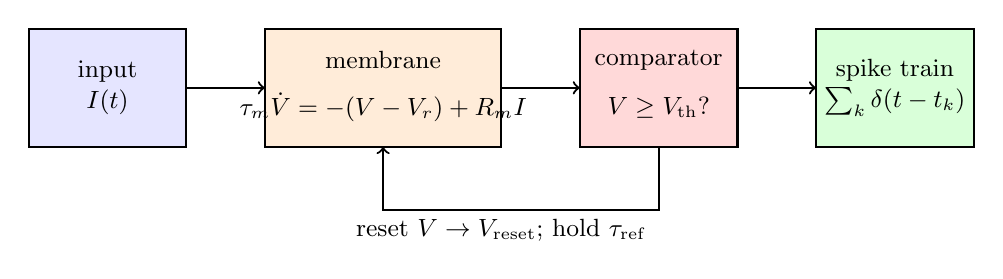
\begin{tikzpicture}[scale=1.0, every node/.style={font=\small}]
  % Input block
  \draw[thick, fill=blue!10] (0,0) rectangle (2.0,1.5);
  \node[align=center] at (1.0,0.75) {input\\$I(t)$};
  % Arrow
  \draw[->, thick] (2.0,0.75) -- (3.0,0.75);
  % RC block
  \draw[thick, fill=orange!15] (3.0,0) rectangle (6.0,1.5);
  \node[align=center] at (4.5,1.1) {membrane};
  \node[align=center] at (4.5,0.5) {$\tau_m \dot{V} = -(V-V_r) + R_m I$};
  % Arrow
  \draw[->, thick] (6.0,0.75) -- (7.0,0.75);
  % Threshold comparator
  \draw[thick, fill=red!15] (7.0,0) rectangle (9.0,1.5);
  \node[align=center] at (8.0,1.1) {comparator};
  \node[align=center] at (8.0,0.5) {$V \ge V_\mathrm{th}$?};
  % Arrow
  \draw[->, thick] (9.0,0.75) -- (10.0,0.75);
  % Spike output block
  \draw[thick, fill=green!15] (10.0,0) rectangle (12.0,1.5);
  \node[align=center] at (11.0,0.75) {spike train\\$\sum_k \delta(t-t_k)$};
  % Reset feedback
  \draw[->, thick] (8.0,0) -- (8.0,-0.8) -- (4.5,-0.8) -- (4.5,0);
  \node[below, align=center] at (6.0,-0.8) {reset $V \to V_\mathrm{reset}$; hold $\tau_\mathrm{ref}$};
\end{tikzpicture}
\caption[Leaky integrate-and-fire block diagram]{The leaky
integrate-and-fire neuron as a signal-processing block. An input
current charges a leaky RC membrane; a comparator emits a spike when
$V$ crosses threshold; the comparator's output feeds back to reset the
membrane and hold it for a refractory period before resuming
integration.}
\label{fig:vol06:ch07:lif-block}
\end{figure}


\textbf{Procedure.}

\begin{enumerate}[leftmargin=*]
\item Implement the LIF model with parameters $\tau_m = 20\,\text{ms}$,
  $V_{\text{rest}} = -65\,\text{mV}$, $V_{\text{th}} = -50\,\text{mV}$,
  $V_{\text{reset}} = -75\,\text{mV}$, $R_m = 10\,\text{M}\Omega$,
  $\tau_{\text{ref}} = 2\,\text{ms}$.
\item Inject a constant current $I_0$ for $1\,\text{s}$. Find the
  threshold current at which the neuron starts firing.
\item Vary $I_0$ above threshold and plot the firing rate as a
  function of $I_0$ (the f-I curve). Identify the saturating regime
  at high $I_0$ where the refractory period limits the firing rate.
\item Add a slow adaptation current that increases after each spike
  and decays with a time constant of $100\,\text{ms}$. Show that the
  neuron now exhibits spike-frequency adaptation under sustained
  input.
\item Drive the neuron with a noisy input current (Gaussian
  white noise) and characterise the firing-rate response.
\end{enumerate}

\textbf{Reference implementation.} The script
\verb|code/lif_neuron.py| in the chapter directory implements all
five steps and produces the f-I curve, the adaptation comparison,
the noisy-input voltage trace, and a textual report of the threshold
current.

\textbf{Deliverable.} A five- to ten-page report with f-I curves with
and without adaptation, a sample voltage trace showing the
spike-and-reset behaviour, source code, and a paragraph identifying
which feature of real neurons the LIF model does and does not
reproduce (it captures the integrate-and-fire dynamics but misses the
spike shape and the rich ionic-channel dynamics of the Hodgkin-Huxley
model).

\textbf{Time.} Four to eight hours.
\end{project}

\section{Exercises}

\subsection*{Calculation}\pathtag{core}

\begin{exercise}
A neuron has $[\text{K}^+]_i = 140\,\text{mM}$ and
$[\text{K}^+]_o = 4\,\text{mM}$ at $310\,\si{\kelvin}$. Compute the
Nernst equilibrium potential for potassium.
\end{exercise}

\paragraph{Solution sketch.}
The Nernst potential is $E_K = (RT/zF) \ln([\text{K}^+]_o /
[\text{K}^+]_i)$ with $z = +1$. At $T = 310\,\si{\kelvin}$,
$RT/F = (8.314 \cdot 310)/96485 = 26.7\,\text{mV}$, so
$E_K = 26.7\,\text{mV} \cdot \ln(4/140)
= 26.7\,\text{mV} \cdot (-3.555)
= -94.9\,\text{mV} \approx -95\,\text{mV}$. The result lies a few
millivolts negative of the typical resting potential because the
membrane is not exclusively permeable to K$^+$; the GHK equation
weighs in the smaller but non-zero permeabilities to Na$^+$ and
Cl$^-$ to give $V_{\text{rest}} \approx -70\,\text{mV}$. See
\cite[ch.~6]{text:v6c07-kandel-principles-2021}.

\begin{exercise}
A mammalian axon has membrane capacitance $1\,\si{\micro\farad}/\text{cm}^2$
and a membrane resistance of $5000\,\Omega\,\text{cm}^2$ in the resting
state. Compute the membrane time constant.
\end{exercise}

\paragraph{Solution sketch.}
The membrane time constant is $\tau_m = R_m C_m =
(5000\,\Omega\,\text{cm}^2)(10^{-6}\,\text{F}/\text{cm}^2) =
5 \times 10^{-3}\,\text{s} = 5\,\text{ms}$. The result places the
axon in the middle of the typical mammalian range ($1$ to
$20\,\text{ms}$). Larger $\tau_m$ means slower integration and
longer temporal summation of synaptic inputs; smaller $\tau_m$ means
faster response but less integration. The time constant is a tunable
parameter of the cell: opening more leak channels reduces $R_m$ and
hence $\tau_m$, sharpening temporal precision at the cost of
sensitivity.

\begin{exercise}
A myelinated axon of $5\,\si{\micro\meter}$ diameter has internodal
distance $1\,\text{mm}$ and conduction velocity $30\,\text{m}/\text{s}$.
Compute the time required for an action potential to jump from one
node to the next.
\end{exercise}

\paragraph{Solution sketch.}
Time per internodal jump $= L/v = (1 \times 10^{-3}\,\text{m})/
(30\,\text{m}/\text{s}) = 3.3 \times 10^{-5}\,\text{s}
= 33\,\si{\micro\second}$. The local regeneration at each node takes
about $0.1\,\text{ms} = 100\,\si{\micro\second}$, so saltatory
conduction is rate-limited by the node-to-node regeneration time,
not by the inter-node transit time. The effective velocity is
$\sim L/\tau_{\text{regen}}$, which for typical mammalian fibres
gives the observed $\sim 30$ to $120\,\text{m/s}$ range
\cite[ch.~6]{text:v6c07-kandel-principles-2021}.

\begin{exercise}
A neuron fires at $50\,\text{Hz}$ for $1\,\text{s}$. With each action
potential the neuron consumes $5 \times 10^8\,\text{ATP}$ molecules.
Compute the total ATP consumption during the burst and convert to
energy in joules.
\end{exercise}

\paragraph{Solution sketch.}
Total ATP $= 50 \times 5 \times 10^8 = 2.5 \times 10^{10}$
molecules. Each ATP hydrolysis yields $\sim 30\,\text{kJ}/\text{mol}$
under cellular conditions (the in-vitro $\Delta G^\circ = -30.5\,\text{kJ}/\text{mol}$
adjusted for typical intracellular [ATP], [ADP], [Pi] gives
$\sim 50$ to $60\,\text{kJ}/\text{mol}$ in vivo). Taking
$50\,\text{kJ}/\text{mol}$:
\[
E = 2.5 \times 10^{10} \times \frac{50 \times 10^3}{6.022 \times 10^{23}}\,\text{J}
\approx 2.1 \times 10^{-9}\,\text{J} \approx 2\,\text{nJ}.
\]
Two nanojoules per second per cell, scaled to the brain's
$\sim 10^{11}$ neurons, gives a brain-wide power of
$\sim 200\,\text{W}$, which overshoots the actual brain power
($\sim 20\,\text{W}$) by a factor of $10$ because most neurons fire
at $\sim 1\,\text{Hz}$, not $50$. Plugging the average rate back in
recovers the observed brain power and verifies the order of magnitude.

\begin{exercise}
A synaptic vesicle contains $5000$ molecules of glutamate. An action
potential at the presynaptic terminal releases $10$ vesicles. Compute
the number of glutamate molecules released and the concentration in
the cleft (volume $\sim 4 \times 10^{-17}\,\text{L}$).
\end{exercise}

\paragraph{Solution sketch.}
Released $= 10 \times 5000 = 5 \times 10^4$ molecules. Concentration
$= 5 \times 10^4 / (6.022 \times 10^{23} \times 4 \times 10^{-17})
\approx 2 \times 10^{-3}\,\text{M} = 2\,\text{mM}$. The cleft
concentration is high (millimolar range) for a short interval
($< 1\,\text{ms}$), saturating ionotropic AMPA receptors briefly. The
high transient concentration is the reason synaptic transmission is
both fast (saturation makes the response time-locked to the cleft
peak) and reliable (saturation makes the response insensitive to small
variations in release).

\begin{exercise}
A typical B-cell repertoire contains $10^{11}$ cells in an adult human
with $10^{10}$ distinct antigen specificities. Compute the average
number of B cells per specificity and the probability that any given
specificity is present in a $1\,\text{mL}$ blood sample
($5 \times 10^6$ B cells per mL).
\end{exercise}

\paragraph{Solution sketch.}
Average B cells per specificity $= 10^{11} / 10^{10} = 10$. In a
$1\,\text{mL}$ sample of $5 \times 10^6$ B cells, the sample fraction
is $5 \times 10^6 / 10^{11} = 5 \times 10^{-5}$. The expected count
per specificity in the sample is $10 \times 5 \times 10^{-5} =
5 \times 10^{-4}$. Modelling occupancy as Poisson, the probability of
finding at least one cell of a given specificity is
$1 - e^{-5 \times 10^{-4}} \approx 5 \times 10^{-4}$. A small blood
draw therefore misses most rare specificities. Concentrating
lymphocytes from large blood volumes or from lymph nodes is essential
for the diagnostic and engineering applications (TCR repertoire
sequencing, adoptive transfer protocols).

\begin{exercise}
The adaptive immune response produces $\sim 10^4$-fold clonal
expansion of antigen-specific T cells in $7\,\text{days}$. Compute
the effective doubling time and compare to the typical cell-cycle
time of $\sim 8\,\text{hours}$ for activated lymphocytes.
\end{exercise}

\paragraph{Solution sketch.}
$10^4 = 2^n$ gives $n = \log_2(10^4) = 4 \log_2 10 \approx 13.3$
doublings. Over $7\,\text{days} = 168\,\text{hours}$, the effective
doubling time is $168/13.3 \approx 12.6\,\text{hours}$. The cell-
cycle time is $\sim 8\,\text{hours}$, so the effective time is
$\sim 1.6\times$ slower, reflecting a $\sim 60\%$ effective fraction
of cells in cycle at any given moment with the remainder in apoptosis,
quiescence, or differentiation into memory. The factor accounts for
the realised expansion rate observed in vivo \cite[ch.~11]{text:v6c07-janeway-immunobiology-2017}.

\subsection*{Derivation}\pathtag{standard}

\begin{exercise}
Derive the Hodgkin-Huxley equation for membrane current as a sum of
sodium, potassium, and leakage components. Identify the role of each
gating variable.
\end{exercise}

\paragraph{Solution sketch.}
The membrane is modelled as a capacitance $C_m$ in parallel with three
ionic conductances (sodium, potassium, leak). Kirchhoff's current law
applied to the membrane gives
$C_m\,dV/dt + I_{\text{ion}} = I_{\text{ext}}$, where
$I_{\text{ion}} = I_{\text{Na}} + I_K + I_L$. Each ionic current is
proportional to the driving force $(V - E_X)$ times the conductance
$g_X(V,t)$. Hodgkin and Huxley fit voltage-clamp data with
$g_{\text{Na}} = \bar{g}_{\text{Na}} m^3 h$ and $g_K = \bar{g}_K n^4$,
where $m, h, n$ each obey first-order kinetics
$dx/dt = (x_\infty(V) - x)/\tau_x(V)$. The variable $m$ is the
sodium-activation gate, controlling the rapid opening of sodium
channels; $h$ is the sodium-inactivation gate, slower than $m$ and
falling on depolarisation, producing the inactivation that ends the
spike; $n$ is the potassium-activation gate, slow to rise and slow to
fall, producing the delayed potassium current that repolarises the
membrane. Substituting and rearranging:
\[
C_m \frac{dV}{dt} = -\bar{g}_{\text{Na}} m^3 h (V - E_{\text{Na}})
                    -\bar{g}_K n^4 (V - E_K)
                    - g_L (V - E_L) + I_{\text{ext}}.
\]
The structure is Equation~\ref{eq:hh}. See
\cite[p.~518--520]{paper:v6c07-hodgkin-huxley-1952}.

\begin{exercise}
Derive the cable equation
$\lambda^2 \partial^2 V/\partial x^2 = \tau_m \partial V/\partial t + (V - V_{\text{rest}})$
for a passive neuronal cable. State the assumptions on the membrane
and the axoplasm.
\end{exercise}

\paragraph{Solution sketch.}
Consider a short cable segment of length $dx$. Assumptions: (i) the
membrane is passive (constant $r_m$, $c_m$); (ii) the axoplasm has
constant axial resistance per unit length $r_a$ and zero
capacitance; (iii) the extracellular space is isopotential
(short-circuited at $V = 0$); (iv) the cable diameter is constant
along the segment. Apply Kirchhoff's current law: the current entering
the segment from the left along the axoplasm equals the current
leaving to the right plus the current crossing the membrane to ground.
Ohm's law for the axial current is
$i_a(x) = -(1/r_a) \partial V/\partial x$. The membrane current per
unit length is $i_m = c_m \partial V/\partial t + (V - V_{\text{rest}})/r_m$.
Conservation gives $\partial i_a/\partial x = -i_m$. Substituting and
rearranging:
\[
\frac{1}{r_a} \frac{\partial^2 V}{\partial x^2}
= c_m \frac{\partial V}{\partial t} + \frac{V - V_{\text{rest}}}{r_m}.
\]
Multiplying through by $r_m$ and identifying $\tau_m = r_m c_m$ and
$\lambda^2 = r_m/r_a$ yields Equation~\ref{eq:cable}. The space
constant $\lambda$ is the characteristic decay length of a steady-state
voltage perturbation; the time constant $\tau_m$ is the membrane
charging time \cite{paper:v6c07-rall-1959}.

\begin{exercise}
Derive the all-or-nothing threshold behaviour of an action potential
from the positive-feedback structure of sodium-channel activation.
Show that the threshold corresponds to the unstable saddle point of
the underlying dynamical system.
\end{exercise}

\paragraph{Solution sketch.}
The HH equations (with gating variables slaved to their voltage-
dependent steady states) reduce on fast time scales to a one-
dimensional flow in $V$. The sodium current introduces a positive-
feedback loop: increasing $V$ opens more $m$, which increases the
inward sodium current, which raises $V$ further. The potassium
current provides delayed negative feedback. On the fast manifold,
$dV/dt = f(V)$ has three zeros at characteristic operating points:
the stable resting state ($V \approx -70\,\text{mV}$), an unstable
intermediate state ($V \approx -50\,\text{mV}$, the threshold), and
the stable peak state ($V \approx +30\,\text{mV}$). The intermediate
zero is the saddle point: any perturbation that pushes $V$ above this
saddle is amplified by the positive feedback and the trajectory shoots
to the peak; any perturbation below dies back to rest. The
all-or-nothing behaviour is therefore the dynamical-systems signature
of the saddle: trajectories above and below the saddle have
qualitatively different fates. On slower timescales the gating
variables relax and the system returns to rest through the recovery
manifold; the cycle is a relaxation oscillation
\cite[ch.~7]{text:v6c07-dayan-abbott-2001}.

\subsection*{Estimation}\pathtag{core}

\begin{exercise}
Estimate the information rate (in bits per second) of a single
cortical neuron firing at $5\,\text{Hz}$ with $1\,\text{ms}$ timing
precision.
\end{exercise}

\paragraph{Solution sketch.}
Divide one second into bins of $\Delta t = 1\,\text{ms}$. Each bin
either contains a spike or does not. The probability of a spike in
a bin is $p = f \Delta t = 5 \times 10^{-3}$. The binary entropy is
$H(p) = -p \log_2 p - (1-p) \log_2 (1-p)$. With $p = 5 \times 10^{-3}$
and $(1-p) \approx 1$:
\[
H(p) \approx -0.005 \log_2 0.005 - 0.995 \log_2 0.995
\approx 0.005 \times 7.64 + 0.995 \times 0.0072
\approx 0.045\,\text{bits/bin}.
\]
At $1000$ bins per second: rate $\approx 45\,\text{bits/s}$. The result
brackets the value measured directly in fly visual neurons
\cite{paper:v6c07-strong-1998}. The estimate assumes statistical
independence across bins; real spike trains have correlations
(refractory periods, bursts) that lower the realised rate by a
factor of $2$ to $3$.

\begin{exercise}
Estimate the total information storage capacity of the human
synaptic network ($10^{14}$ synapses, with each synaptic strength
discriminable into $\sim 10$ levels).
\end{exercise}

\paragraph{Solution sketch.}
With $10^{14}$ synapses each at $\log_2 10 \approx 3.3$ bits, the
storage capacity is
$\sim 10^{14} \times 3.3 = 3 \times 10^{14}\,\text{bits} = 40\,\text{TB}$.
The number compares favourably with a modern flash storage device
($\sim 1$ to $10\,\text{TB}$) and is consistent with the order-of-
magnitude estimates of \cite[ch.~67]{text:v6c07-kandel-principles-2021}.
The estimate ignores stronger constraints: synaptic weights are
not independent (correlations across nearby synapses reduce effective
capacity by a factor of $5$ to $10$); some synapses store no
long-term information (the highly plastic ones are written and
overwritten on hourly to daily timescales); and not all bits are
addressable for retrieval. Realistic capacity is plausibly
$1$ to $10\,\text{TB}$.

\begin{exercise}
Estimate the time required for a naive T cell to find its cognate
antigen in a $1\,\text{mL}$ lymph node, given a typical T-cell
swimming velocity of $\sim 10\,\si{\micro\meter}/\text{min}$.
\end{exercise}

\paragraph{Solution sketch.}
The T cell performs a random walk through the lymph node, scanning
dendritic cells for cognate peptide-MHC. The lymph-node volume is
$1\,\text{mL} = 10^{12}\,\si{\micro\meter}^3$. The T cell moves at
$10\,\si{\micro\meter}/\text{min}$ for a few minutes between
direction changes, giving a diffusion coefficient
$D \sim L^2/\tau \sim (50\,\si{\micro\meter})^2/3\,\text{min}
\sim 800\,\si{\micro\meter}^2/\text{min}$. The mean time to
encounter one of $n_{\text{DC}} \sim 10^7$ dendritic cells in the
lymph node, each acting as a target sphere of radius
$r \sim 10\,\si{\micro\meter}$, is given by the Smoluchowski rate
$\kappa = 4 \pi D r n_{\text{DC}} / V$. Plugging in:
$\kappa \sim 4 \pi \times 800 \times 10 \times 10^7 / 10^{12}
\approx 1\,\text{min}^{-1}$, so the encounter time is $\sim 1\,\text{min}$.
Each encounter lasts $\sim 30\,\text{minutes}$ for non-cognate cells,
shorter for cognate. The realised search time over a $24$-hour
lymph-node residence is consistent with the observed kinetics of
T-cell activation.

\begin{exercise}
Estimate the number of distinct antigens that the adaptive immune
system can recognise in a typical mammalian host. Compare to the
estimated diversity of pathogen antigens encountered in a lifetime.
\end{exercise}

\paragraph{Solution sketch.}
The realised TCR repertoire in a single human is $\sim 10^7$ to
$10^8$ distinct clonotypes (sampled from a combinatorial space of
$10^{15}$ to $10^{18}$ possibilities). The realised B-cell repertoire
is similar before affinity maturation, broader after. Each receptor
recognises a small region of antigen space (with cross-reactivity to
$\sim 10^2$ to $10^4$ related peptides for typical TCRs), so the
total antigen coverage is $\sim 10^9$ to $10^{12}$ distinct
peptides recognisable, several orders of magnitude greater than the
$\sim 10^6$ to $10^8$ antigenically distinct molecular species
encountered in a typical lifetime. The repertoire is therefore
over-engineered for the encountered antigen diversity, providing a
substantial safety margin against novel pathogens and against
pathogen evolution.

\subsection*{Simulation}\pathtag{mastery}

\begin{exercise}
Implement the full Hodgkin-Huxley model in code and reproduce a
single action potential. Vary the leak conductance and identify the
range over which action potentials are still produced.
\end{exercise}

\paragraph{Solution sketch.}
The reference implementation is \verb|code/hodgkin_huxley.py| in the
chapter directory. With the canonical parameters and a brief
$10\,\si{\micro\ampere}/\text{cm}^2$ stimulus, a single action
potential is produced. Sweeping $g_L$ from $0.05$ to $0.8\,\text{mS}/\text{cm}^2$
shows that for $g_L \lesssim 0.5$, the action potential fires; for
larger $g_L$, the leak current shunts the inward sodium current
before the regenerative threshold is reached and the potential
collapses sub-threshold. The result is the classical leak-shunt
threshold and explains why pharmacological agents that increase
membrane leak (some anaesthetics, K$^+$-channel openers) suppress
excitability.

\begin{exercise}
Simulate a small recurrent network of $100$ leaky integrate-and-fire
neurons with random connectivity. Identify the parameter regimes in
which the network sustains asynchronous activity, synchronous
oscillations, or quiescence.
\end{exercise}

\paragraph{Solution sketch.}
Extend the LIF code to $N = 100$ neurons with sparse random
connectivity ($p_{\text{conn}} = 0.1$) and a fraction $f_{\text{inh}}
= 0.2$ inhibitory. The three regimes correspond to: (i) quiescence,
when external drive is below the threshold-crossing rate
($I_{\text{ext}} < I_{\text{th}}$); (ii) asynchronous irregular
activity, when excitatory and inhibitory inputs roughly cancel,
producing Poisson-like spiking with mean rate set by the residual
input (the Brunel 2000 regime); (iii) synchronous oscillations, when
recurrent excitation dominates inhibition or when the inhibitory
delay produces a fixed-period feedback loop. The Brunel paper is the
canonical analysis; the f-I curve from the project supplies the
local nonlinearity.

\subsection*{Design}\pathtag{standard}

\begin{exercise}
Design a closed-loop brain-machine interface that decodes the motor
intention from cortical neural activity and controls a prosthetic
arm. Specify the recording technology (intracortical electrode array,
ECoG, EEG), the decoding algorithm, and the feedback latency.
\end{exercise}

\paragraph{Discussion.}
A workable architecture (current as of 2024): record from a
$96$-channel intracortical array (Utah array, Blackrock) implanted in
primary motor cortex, sampling at $30\,\text{kHz}$; threshold-cross
spike detection in firmware; population decoder is a Kalman filter
on the smoothed firing-rate vector mapping to end-effector velocity in
three degrees of freedom. End-to-end loop latency target: $50\,\text{ms}$
(neural-to-motor command), within the natural sensorimotor loop time.
Failure modes to address: electrode-tissue interface degradation
(impedance creep, glial encapsulation) limiting recording lifetime to
$1$ to $5\,\text{years}$; decoder drift as the recorded population
changes day to day, requiring daily recalibration; and the absence of
proprioceptive feedback to the user, which can be addressed by visual
feedback or by direct cortical microstimulation of somatosensory
cortex (in research demonstrations). ECoG (subdural surface
electrodes) offers a longer-lived but lower-resolution alternative;
EEG (scalp electrodes) is non-invasive but too noisy for fine motor
decoding.

\begin{exercise}
Design a vaccine for a novel pathogen given its genomic sequence.
Specify the antigen choice, the platform (mRNA, viral vector,
protein subunit, attenuated live), the adjuvant, and the
dose-response study.
\end{exercise}

\paragraph{Discussion.}
A workable approach (current as of 2024): identify a conserved
surface protein essential for pathogen entry (the SARS-CoV-2 spike
protein is the template); confirm the antigen by in vitro
neutralisation; select an mRNA platform for development speed,
encoding a stabilised pre-fusion conformation of the antigen and
delivered in lipid nanoparticles; use no exogenous adjuvant, since
the lipid nanoparticles are themselves immunogenic; conduct a
dose-finding Phase 1 ($n \sim 100$, two-dose regimen at $25$ to
$100\,\si{\micro\gram}$) to characterise the neutralising-antibody
titre response and the safety profile; then Phase 2 ($n \sim 1000$
to confirm immunogenicity in subpopulations); then Phase 3
($n \sim 30\,000$ to power a clinical-endpoint efficacy estimate).
Reference: the BNT162b2 development programme
\cite{paper:v6c07-mrna-pfizer-2020}.

\begin{exercise}
Design a chimeric antigen receptor T cell (CAR-T) therapy targeting
a specific tumour cell-surface marker. Specify the antigen-recognition
domain, the signalling domains (CD3$\zeta$, CD28, 4-1BB), and the
expected off-target risks.
\end{exercise}

\paragraph{Discussion.}
A workable construct (the FDA-approved Kymriah for B-cell ALL is the
template): anti-CD19 single-chain antibody (scFv) as the
antigen-binding domain; a hinge and transmembrane region; an
intracellular signalling cassette of $4$-$1$BB co-stimulation
followed by CD3$\zeta$ activation; expression from a lentiviral
vector in the patient's own T cells, ex vivo. Off-target risks:
(i) on-target off-tumour toxicity: CD19 is expressed on all B cells,
so CAR-T therapy ablates normal B cells along with the tumour,
requiring lifelong immunoglobulin replacement; (ii) cytokine release
syndrome (CRS): massive T-cell activation produces life-threatening
inflammation, managed with anti-IL-6 (tocilizumab) and steroids;
(iii) neurotoxicity (ICANS): poorly understood but life-threatening
in a fraction of patients; (iv) loss of CD19 expression by the tumour
(antigen escape) producing relapse. The clinical pipeline addresses
each through gating-construct design and through redirection to
multiple antigens \cite{paper:v6c07-june-cart-2018}.

\subsection*{Diagnosis and reverse engineering}\pathtag{core}

\begin{exercise}
A patient presents with rapidly progressive weakness over hours,
ascending from the feet. Identify the most likely mechanism class
(demyelinating polyneuropathy, peripheral nerve), the expected
electrophysiology findings, and one diagnostic test.
\end{exercise}

\paragraph{Discussion.}
The clinical picture (rapidly progressive ascending weakness in a
previously well adult) is the textbook presentation of Guillain-Barr\'{e}
syndrome (GBS), an acute inflammatory demyelinating polyneuropathy
that classically follows a viral or \emph{Campylobacter jejuni}
gastrointestinal illness by one to four weeks (molecular mimicry
mechanism). Expected nerve-conduction findings: marked slowing of
motor conduction velocities (target nerves $< 30\,\text{m/s}$ versus
normal $\sim 50\,\text{m/s}$), prolonged distal latencies, and
conduction block in motor fibres; F-wave latencies prolonged or
absent. Diagnostic test: lumbar puncture showing albuminocytological
dissociation (raised cerebrospinal-fluid protein with a normal cell
count). Treatment: intravenous immunoglobulin (IVIG) or plasma
exchange to clear the cross-reacting antibodies; supportive care
(ventilation if the diaphragm is involved). The presentation
illustrates the molecular-mimicry mechanism class and the engineering
response of antibody removal.

\begin{exercise}
A patient with rheumatoid arthritis develops persistent joint
inflammation despite immunosuppression with methotrexate. Identify
two possible engineering interventions (anti-TNF biologic, JAK
inhibitor, B-cell depletion) and one diagnostic test that would
guide the choice.
\end{exercise}

\paragraph{Discussion.}
Two interventions: (i) anti-TNF biologic (infliximab, etanercept,
adalimumab) targets the central inflammatory cytokine of RA;
expected response within weeks. (ii) anti-CD20 B-cell depletion
(rituximab) targets the autoantibody-producing B-cell pool; expected
response within months and longer-lived. A guiding diagnostic test:
serology for rheumatoid factor and anti-citrullinated protein
antibodies (anti-CCP). Patients with high anti-CCP titres typically
respond well to B-cell depletion; seronegative patients respond
preferentially to anti-TNF or JAK inhibition. The choice illustrates
the substitution principle: when one immunosuppressive mechanism
fails, switch to a different mechanism rather than escalate the same
class.

\begin{exercise}
A patient develops repeated bacterial pneumonias from low-virulence
organisms throughout childhood. Identify the most likely class of
immunodeficiency (humoral, with low immunoglobulin levels) and propose
the principal therapeutic response.
\end{exercise}

\paragraph{Discussion.}
The pattern (recurrent pneumonias from encapsulated organisms such
as \emph{Streptococcus pneumoniae} or \emph{Haemophilus influenzae})
points to a humoral immunodeficiency: the patient cannot mount
effective antibody responses to polysaccharide capsular antigens.
The differential includes common variable immunodeficiency (CVID),
X-linked agammaglobulinaemia (Bruton's tyrosine kinase mutation,
absent B cells), or selective IgA/IgG-subclass deficiency. Confirm
by quantitative serum immunoglobulins and B-cell flow cytometry.
The principal therapeutic response is replacement: monthly intravenous
or subcutaneous immunoglobulin (IVIG/SCIG) at $400$ to
$600\,\text{mg/kg}$, raising the trough IgG level above the
infection-protection threshold ($\sim 5\,\text{g/L}$). Prophylactic
antibiotics may also be used. The case illustrates the engineering
response of replacement when the defective component cannot be
restored.

\subsection*{Failure analysis}\pathtag{core}

\begin{exercise}
A patient with type-1 diabetes loses pancreatic $\beta$-cell function
over months. Identify the mechanism class (autoimmune destruction by
self-reactive T cells), the specific antigens involved (insulin, GAD65),
and the therapeutic engineering response.
\end{exercise}

\paragraph{Discussion.}
The mechanism is autoimmune attack on islet $\beta$-cells by self-
reactive CD8$^+$ T cells, with autoantibodies against pre-proinsulin,
glutamic acid decarboxylase 65 (GAD65), and islet antigen 2 (IA-2)
as serological markers and predictors of progression. The therapeutic
response (current as of 2024) is replacement: exogenous insulin
delivered subcutaneously or via continuous subcutaneous insulin
infusion (CSII), increasingly integrated with continuous glucose
monitors and closed-loop algorithms (``artificial pancreas''
hybrid-closed-loop systems are now FDA-approved). For at-risk
patients identified by autoantibody screening, the anti-CD3 antibody
teplizumab (FDA-approved 2022) can delay clinical onset by $2$ to
$3\,\text{years}$ through transient depletion of activated T cells.
Islet transplantation and stem-cell-derived $\beta$-cell replacement
are under development but not yet standard of care.

\begin{exercise}
A patient receiving an anti-CTLA-4 checkpoint inhibitor for melanoma
develops severe colitis. Identify the mechanism class
(immune-mediated adverse event from broad-spectrum T-cell activation)
and the engineering response (steroids, IL-6 receptor antagonist,
discontinuation of immunotherapy).
\end{exercise}

\paragraph{Discussion.}
The mechanism is the predictable consequence of CTLA-4 blockade:
removing one of the brakes on T-cell activation produces broader
T-cell activation against both tumour and self-tissue. The colon is
particularly vulnerable because of its constant exposure to luminal
antigens. The engineering response is graded: (i) low-dose loperamide
and supportive care for mild diarrhoea; (ii) high-dose corticosteroids
(prednisone $1$ to $2\,\text{mg/kg}$) for moderate to severe colitis;
(iii) anti-TNF (infliximab) or anti-$\alpha_4 \beta_7$ (vedolizumab)
for steroid-refractory cases; (iv) permanent discontinuation of the
checkpoint inhibitor in life-threatening cases. The case illustrates
that engineering interventions in the immune system carry
discrimination side-effects: dropping a brake increases response
against intended and unintended targets simultaneously
\cite{paper:v6c07-allison-2018-nobel}.

\subsection*{Judgment}\pathtag{standard}

\begin{exercise}
A press release announces a ``brain-computer interface that reads
thoughts directly''. Identify the engineering claims (single-trial
decoding of complex thought, generalisation across subjects, signal
acquisition method) and write a one-paragraph reply asking the
researchers to specify the actual capability.
\end{exercise}

\paragraph{Discussion.}
A useful reply asks four questions. (i) What is the bandwidth of the
decoded output? Current intracortical BMIs achieve typing at $\sim 10$
to $40\,\text{characters/min}$, less than $0.5\,\text{bits/s}$ after
correction. (ii) Is the system per-subject calibrated or
subject-general? Typically per-subject, with daily recalibration.
(iii) What does the system decode: motor intention (well-developed,
achieving the cited typing rates), or semantic content (much more
limited, with current work decoding short imagined sentences with
considerable error)? (iv) What is the implant footprint and the
expected longevity of the recording? An honest answer would tighten
``reads thoughts directly'' to ``decodes a low-bandwidth motor or
phonemic intention from a multi-electrode recording in a specific
cortical region, in a calibrated single subject, over hours to
months.''

\begin{exercise}
A vaccine sceptic argues that vaccines are ``unnatural'' because they
introduce antigens directly into the body. Identify the engineering
function the argument misses (vaccines establish adaptive memory
without the disease risk of natural infection) and write a
one-paragraph reply explaining the trade-off in engineering terms.
\end{exercise}

\paragraph{Discussion.}
The engineering reply: a vaccine and a natural infection both train
the adaptive immune system to recognise a pathogen. The natural
infection delivers the antigen alongside the pathogen's full
replication machinery, including the components that cause disease;
the vaccine delivers the antigen with the disease-causing components
removed or attenuated. The trade-off is therefore: accept a small,
quantifiable risk from the vaccine (which has been measured in
millions of recipients and is in the range $10^{-5}$ to $10^{-6}$ for
serious adverse events for most modern vaccines) to avoid the larger
and harder-to-quantify risk from natural infection (which for many
target diseases includes mortality risks in the percent range and
chronic-sequelae risks several percent more). The argument from
naturalness conflates the source of the antigen with its
engineering function; the engineering reading is that the source is
incidental and the function is what matters.

\begin{exercise}
A textbook describes the nervous system as ``the body's computer''.
Identify two ways in which the computer metaphor is accurate
(information processing, parallel architecture) and two ways in
which it is misleading (the brain is not digital, and its memory is
not addressable in the way a computer's is).
\end{exercise}

\paragraph{Discussion.}
Accurate: (i) both transform inputs into outputs through structured
computation; (ii) both are organised hierarchically into layered
processing stages with feedback and feed-forward pathways. Misleading:
(i) the brain operates with mixed analog-digital signalling
(subthreshold integration is analog; spike output is digital;
neuromodulation is graded), while a computer is digital throughout;
(ii) brain memory is content-addressable and distributed (no
specific neuron stores ``grandmother''; the representation is
distributed across populations), while computer memory is location-
addressable; (iii) the brain learns continuously and changes its
own connection weights, while a computer's hardware is fixed and
its software changes only under explicit programmer instruction;
(iv) the brain operates with massive metabolic constraints
($\sim 20\,\text{W}$ for $\sim 10^{11}$ elements) that dominate its
design choices, while computers use orders of magnitude more energy
per operation. The metaphor is a useful approximation at the
information-processing level and a misleading one at every level
below.

\begin{exercise}
A start-up advertises a ``general-purpose immunotherapy'' that uses
a single CAR-T construct to treat any cancer. Identify the engineering
challenges the claim must address (tumour heterogeneity, antigen
specificity, on-target off-tumour toxicity) and write a one-paragraph
reply identifying the assumption most likely to be over-claimed.
\end{exercise}

\paragraph{Discussion.}
The over-claim is that a single antigen target generalises across
tumour types. In reality each tumour expresses a specific set of
surface markers; CAR-T therapy requires the target to be (i) reliably
present on the tumour, (ii) absent or sparse on essential normal
tissue, and (iii) maintained through clonal evolution of the tumour.
CD19 satisfies these for B-cell malignancies (the entire B-cell
compartment can be ablated and replaced by immunoglobulin therapy);
solid-tumour antigens that satisfy all three conditions are rare and
under active development (mesothelin, GPC3, claudin-18.2). The reply:
ask the start-up which specific antigen the construct targets, what
the on-target off-tumour profile is, and how the construct handles
antigen escape; if the answers are vague, the claim is unsupported
\cite{paper:v6c07-june-cart-2018}.

\begin{exercise}
A press release announces an experimental therapy that ``cures
autoimmune disease by retraining the immune system''. Identify the
mechanism claim (restoration of tolerance) and write a one-paragraph
reply asking the company to specify which tolerance mechanism is
being restored (central versus peripheral, deletion versus regulatory
T cell expansion).
\end{exercise}

\paragraph{Discussion.}
The reply requests specificity along four axes. (i) Which tolerance
mechanism is invoked: central (thymic deletion of self-reactive
clones), peripheral (Treg-mediated suppression, anergy, activation-
induced cell death), or both? (ii) Is the mechanism antigen-specific
(targeted to the disease-driving autoantigen) or broad-spectrum (like
conventional immunosuppression)? Antigen-specific tolerance is the
holy grail and the much rarer engineering achievement. (iii) What is
the durability: does the patient need re-treatment, and on what
schedule? (iv) What are the safety endpoints: have the developers
monitored for incident infections and incident cancers, both of which
follow from any breach of immune surveillance? Vague answers indicate
either a poorly characterised mechanism or a mature one that has
been over-marketed.

\begin{exercise}
A reader argues that artificial neural networks demonstrate that
biological neurons are well-modelled by simple weighted sums and
non-linearities. Identify two engineering distinctions the argument
overlooks (spike timing as a signalling variable, dendritic
nonlinearities that compute locally before reaching the soma) and
write a one-paragraph reply situating the artificial-neural-network
abstraction relative to biological neurons.
\end{exercise}

\paragraph{Discussion.}
Artificial neural networks abstract biological neurons to a scalar
activation (analogous to firing rate) and a sigmoidal or ReLU
non-linearity; they ignore (i) spike timing, which biological systems
exploit for synchrony detection, oscillation-locked coding, and
phase-precession-based positional information; (ii) dendritic
computation, where individual dendritic branches integrate inputs
non-linearly (through NMDA receptors, calcium spikes, and active
sodium channels in dendrites) and present preprocessed signals to the
soma; (iii) neuromodulation, where global signals (dopamine,
noradrenaline, acetylcholine) reshape effective gain and learning
rates; (iv) Dale's principle, where each biological neuron releases
one transmitter (excitatory or inhibitory) rather than mixing signs
within a single unit. The artificial network is a useful abstraction
for a class of computational tasks (and a celebrated engineering
success in its own right); it is not a faithful model of biological
neurons in the way that, for instance, the Hodgkin-Huxley equations
are.
